\documentclass[11pt]{article}

% --- Packages essentiels ---
\usepackage[a4paper,margin=1.8cm]{geometry}
\usepackage[english]{babel}
\usepackage{amsmath, amssymb}
\usepackage{graphicx}
\usepackage{enumitem}
\usepackage{pdfpages}
\usepackage{tikz}
\usetikzlibrary{arrows.meta}
\usepackage{xcolor}
\usepackage{soul}   
\usepackage{comment}
\usepackage{textcomp}
\usepackage{float}
\usepackage{wrapfig}
\usepackage{caption}
\usepackage{subcaption}
\usepackage{eurosym}
\usepackage{epstopdf}
\epstopdfsetup{update, outdir=./}
\usepackage{booktabs}
\usepackage{array}
\usepackage{tabularx}
\usepackage{hyperref}
\usepackage{titlesec}
\usepackage{setspace}
\usepackage{fancyhdr}
\usepackage{ragged2e}
\usepackage{todonotes}
\usepackage{siunitx}
\setlength{\parindent}{0pt}

% --- Couleur EPFL ---
\definecolor{EPFLred}{RGB}{213, 0, 50}

% --- Interline ---
\singlespacing

% --- Style des titres ---
\titleformat{\section}
  {\large\bfseries}
  {\thesection}{1em}{\vspace{0.3em}}

\titleformat{\subsection}
  {\bfseries}{\thesubsection}{1em}{}

% --- Header & Footer ---
\pagestyle{fancy}
\fancyhf{}
\rhead{\small EPFL}
\lhead{\small Economic growth and sustainability II}
\cfoot{\thepage}

\begin{document}

% -------------------------------------------------
% CONTENU
% -------------------------------------------------

\begin{titlepage}
    \begin{tikzpicture}[remember picture,overlay]
        % Bande verticale rouge
        \fill[red] (current page.north west) rectangle
        ([xshift=3cm]current page.south west);

% Logo EPFL dans la bande
    \node[anchor=north east]
        at ([xshift=-0.7cm,yshift=-1cm]current page.north east)
        {
\includegraphics[width=8cm]{Image/Logo/epfl.png}};
    \end{tikzpicture}

    \vspace*{3.8cm}

    % Contenu à droite
    \hspace*{1.5cm}
    \begin{minipage}{0.9\textwidth}
    \begin{flushright}
        {\Huge  \textbf{CO$_2$ Emissions of Copper Production in Chile}}\\[0.4cm]
        {\Large Economic growth and sustainability}\\[1.2cm]
    
        \rule{0.65\linewidth}{0.6pt}\\[1.2cm]
    
        {\Large \textsc{École Polytechnique Fédérale de Lausanne}}\\[2.2cm]
    
        {\normalsize \textit{Authors / Students :}}\\[0.3cm]
    
        {\Large\textbf{
            Victoria Nene (364043)\\
            Léonard Rambeau (362474)\\
            Edoardo Maserati (363595)\\
            Ismail Essaidi (341008)
        }}\\[1.8cm]
    
        {\normalsize \textit{Teacher: Philippe Thalmann}}\\[0.3cm]
        {\normalsize \textit{Supervisor: Gino Baudry}}\\[0.3cm]
    
        {\large \today}
    \end{flushright}
    \end{minipage}

\end{titlepage}
\tableofcontents
\newpage

\section{Introduction}
\pagenumbering{arabic}
	The global transition toward a low-carbon economy is expected to significantly increase the demand for critical minerals required for renewable energy systems, electric vehicles, electricity grids, and energy storage technologies. Among these materials, copper occupies a particularly important position due to its excellent electrical and thermal conductivity. According to the International Energy Agency (IEA), electric vehicles require approximately 2.5 times more copper than conventional internal combustion vehicles \cite{IEA2021}. Renewable electricity infrastructures, battery storage systems, and modern power grids also rely heavily on copper-intensive technologies. As a result, several studies project a substantial increase in copper demand under global decarbonization scenarios \cite{Watari2020}.

However, this growing dependence on copper also creates an important environmental challenge. While copper is essential for electrification and renewable energy deployment, its extraction and processing remain highly energy-intensive activities requiring large quantities of fuel and electricity \cite{Norgate2010}. Consequently, the expansion of copper production may also increase greenhouse gas emissions and environmental pressures associated with mining activities.

\subsection{Chilean Context and Decarbonization Challenges}

Chile plays a central role in this global challenge as the world’s largest copper producer, accounting for more than 25\% of global copper production \cite{CochilcoWebsite2025}. The mining sector represents a fundamental component of the Chilean economy and contributes significantly to national exports, industrial activity, and public revenues. Copper extraction and processing therefore constitute both a major economic opportunity and an important environmental challenge for the country.

 \begin{figure}[H]
     \centering
     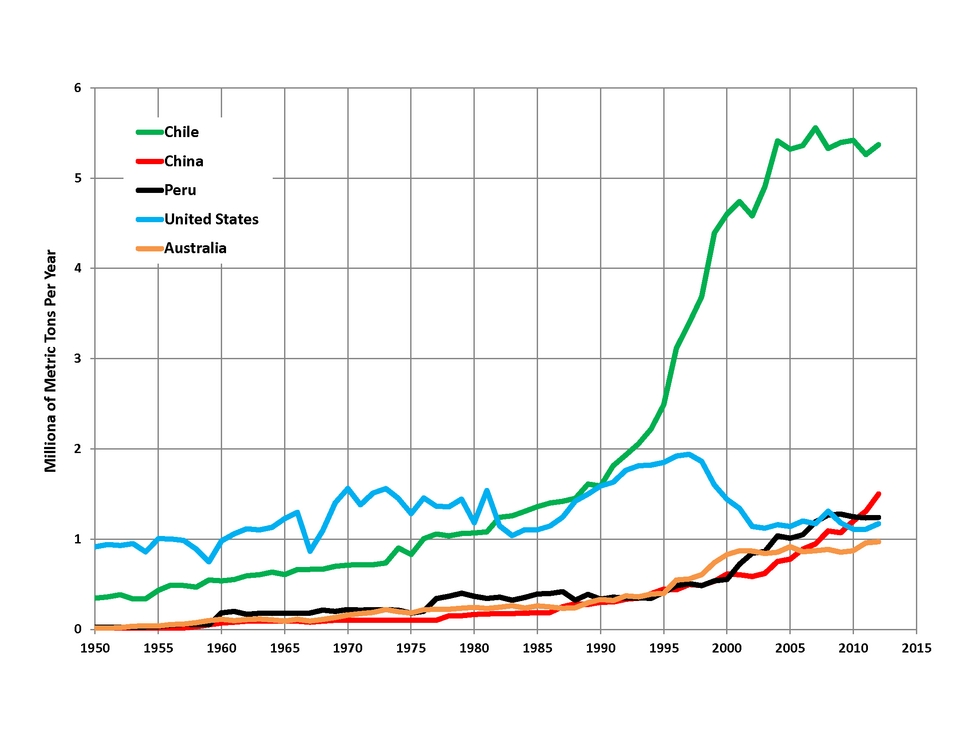
\includegraphics[width=0.8\linewidth]{Figures/image.png}
     \caption{Evolution of copper mine production in the world’s main producing countries between 1950 and 2015, measured in million metric tons per year. Chile experienced the most significant production growth over the period, consolidating its position as the world’s leading copper producer.}
     \label{fig:placeholder}
 \end{figure}

At the same time, Chile has established ambitious climate objectives aimed at achieving carbon neutrality by 2050 \cite{CAT2020}. Over the last decade, the country has rapidly expanded renewable electricity generation, particularly through solar and wind energy development. These transformations are especially relevant for the mining sector because electricity generation strongly influences the carbon footprint associated with copper production. As a result, the Chilean copper industry increasingly stands at the intersection between industrial development, resource extraction, and climate policy.

\subsection{Copper Production Chain and Scope of the Study}

Copper production involves several successive industrial stages that transform low-grade ore into high-purity metal. Depending on the ore type and extraction route, the production chain generally includes mining, crushing, grinding, concentration, smelting, refining, and electro-winning processes. These stages differ significantly in terms of energy requirements, fuel consumption, and electricity intensity.

Open-pit mining operations rely heavily on diesel-powered machinery for extraction and transportation activities, while mineral processing stages such as grinding, concentration, and electro-winning require large amounts of electricity. Smelting and refining operations are also particularly energy-intensive due to the high temperatures required for pyrometallurgical processes.

 \begin{figure}[H]
    \centering
    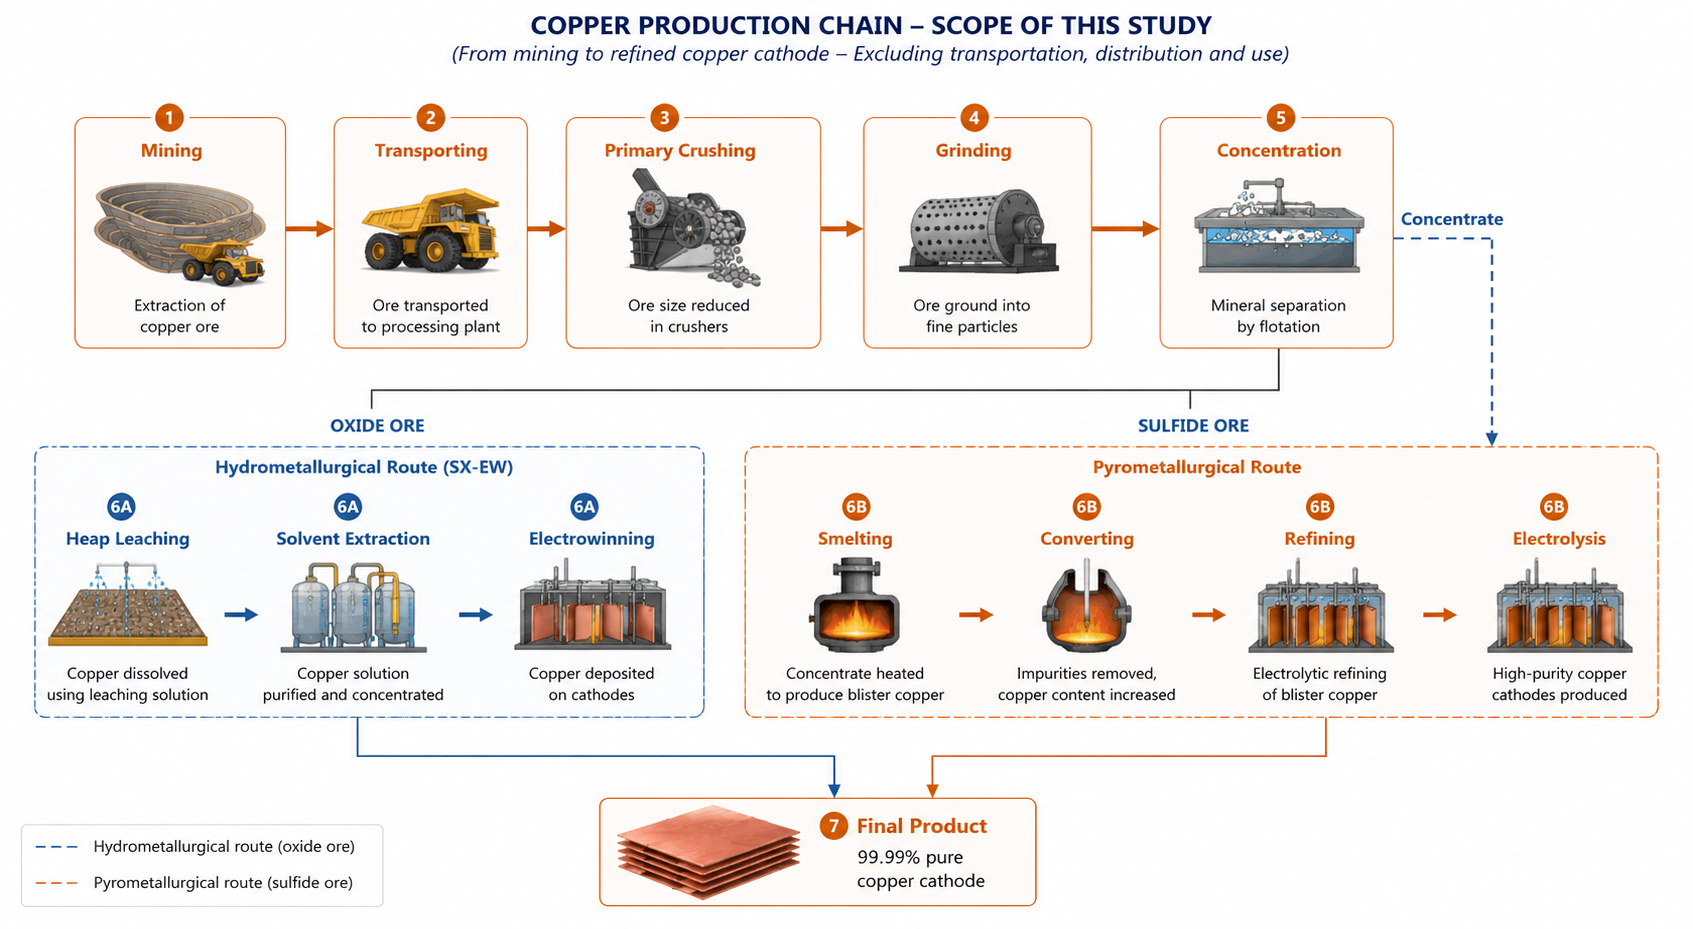
\includegraphics[width=1\linewidth]{Figures/Copper_production_chain_flowchart.png}
    \caption{Simplified representation of the copper production chain considered within the scope of this study. The figure illustrates the main industrial stages involved in transforming copper ore into 99.99\% pure copper cathodes through hydrometallurgical (SX-EW) and pyrometallurgical routes.}
    \label{fig:copper_process}
\end{figure}

Figure~\ref{fig:copper_process} illustrates the main stages of copper production considered within the scope of this study. Depending on the ore type, copper extraction follows either a hydrometallurgical route for oxide ores or a pyrometallurgical route for sulfide ores, both leading to the production of refined copper cathodes. The analysis focuses on the industrial extraction and processing chain, including mining, transportation within mining operations, crushing, concentration, smelting, refining, and electro-winning processes. Downstream stages such as commercialization, international transportation, manufacturing, product use, and end-of-life recycling are excluded from the system boundary. This scope allows the study to concentrate specifically on the industrial activities directly responsible for energy consumption and CO$_2$ emissions associated with copper production.

\subsection{Research Objectives and Methodological Approach}

Despite growing research on mining sustainability, understanding the evolution of CO$_2$ emissions in copper production remains challenging because emissions result from several interacting geological, technological, and energy-related factors. Existing studies often focus on specific aspects of mining decarbonization, such as renewable electricity integration or energy efficiency improvements, but fewer studies analyse how these different drivers jointly influence the evolution of emissions over time.

In this work, we analyse the evolution of CO$_2$ emissions in the Chilean copper mining industry using an IPAT-based decomposition framework. The study focuses on the respective roles of production growth, ore grade evolution, energy consumption, and the distinction between direct emissions from fuel combustion and indirect emissions associated with electricity use. The analysis relies on industrial datasets published by the Chilean Copper Commission (Cochilco), including production, ore grades, energy consumption, and greenhouse gas emissions by process type.

\subsection{Research Questions}

This report aims to answer the following questions:

\begin{itemize}
    \item How have CO$_2$ emissions associated with Chilean copper production evolved over time?

    \item To what extent have production growth, ore grade decline, energy consumption and carbon intensity influenced these emissions?

    \item How can electrification and the decarbonization of Chile’s electricity system contribute to reducing the environmental impact of copper production?
\end{itemize}

% Copper has become one of the most strategic materials in the global effort to reduce greenhouse gas emissions and transition toward a low-carbon economy. Due to its excellent electrical and thermal conductivity, copper is essential for renewable energy technologies, electric vehicles, electrical grids, and energy storage systems. Nevertheless, the extraction and processing of copper require large amounts of energy, making the industry itself a significant source of CO$_2$ emissions. This creates an important contradiction: while copper is indispensable for decarbonization, its production contributes to environmental pollution.

% A central actor in this global challenge is Chile, a South American country that possesses the world’s largest copper reserves and remains the leading producer of copper worldwide. Chile alone accounts for approximately 20\% of global copper reserves and contributes more than 27\% of world copper production. The mining sector is therefore fundamental to the Chilean economy, generating a substantial share of national GDP, exports, and public income. However, the environmental impact of this activity is considerable. Copper extraction in Chile is highly energy-intensive, particularly because ore grades have progressively declined and mining operations have expanded to greater depths. Consequently, mining activities generate significant greenhouse gas emissions. At the same time, Chile benefits from exceptional renewable energy potential, especially in solar and wind energy, which could support the decarbonization of mining operations in the future.

% In this work, we analyse the main drivers of CO$_2$ emissions in the Chilean copper mining industry using an IPAT-based decomposition framework. The study aims to distinguish the relative influence of production growth, ore grade decline, energy intensity, fuel consumption, and electricity-related emissions on the evolution of total greenhouse gas emissions. Particular attention is given to the separation between direct emissions from fuel combustion and indirect emissions associated with electricity use. The analysis focuses on the Chilean copper extraction and processing sector and relies on industrial data published by the Chilean Copper Commission (Cochilco), including production, ore grades, energy consumption, and greenhouse gas emissions by process type.

% \vspace{1em}
% \vspace{1em}
% \subsection{The importance of Copper extraction for Chile's economy}

% Chile has established many climate objectives aimed at helping the global transition toward a low-carbon economy while also addressing the environmental impacts associated with its resource-intensive industries, particularly industries such as mining and copper production. According to the Climate Action Tracker(put ref), Chile’s updated Nationally Determined Contribution (NDC) commits the country to limiting greenhouse gas emissions to a maximum of 95 MtCO$_2$e by 2030 and maintaining a cumulative emissions budget of no more than 1,100 MtCO$_2$e for the 2020–2030 period. The country also plans to ensure that national emissions peak no later than 2025, after which a gradual reduction trajectory should begin. In the longer term, Chile has legally committed, through its Climate Change Framework Law, to achieving carbon neutrality by 2050. To accomplish these goals, Chile is focusing heavily on expanding renewable energy generation, especially solar and wind power, which are particularly important given the country’s exceptional natural resources in the Atacama Desert and coastal regions. The government is also pursuing the gradual phase-out of coal-fired power plants ( a reformuler) , promoting electrification and electromobility, increasing energy efficiency across industrial sectors, and strengthening climate resilience and adaptation measures. Forest conservation and reforestation policies are another central component of Chile’s strategy because natural carbon sinks (plus de details?) are expected to play a major role in offsetting emissions. Furthermore, Chile aims to modernize its mining sector by encouraging cleaner production methods, improving water management, reducing transportation emissions, and increasing the use of renewable electricity in copper extraction and refining processes. These goals are especially significant because Chile is the world’s largest copper producer, and copper is essential for renewable technologies such as electric vehicles, batteries, wind turbines, and power grids. The Climate Action Tracker evaluates Chile’s climate targets as “Almost sufficient,” meaning that while the country has made important progress and its policies are relatively ambitious compared to many nations, additional measures and stronger emission reductions are still necessary for full alignment with the Paris Agreement’s objective of limiting global warming to 1.5°C.
%  \begin{figure}[H]
%     \centering
%     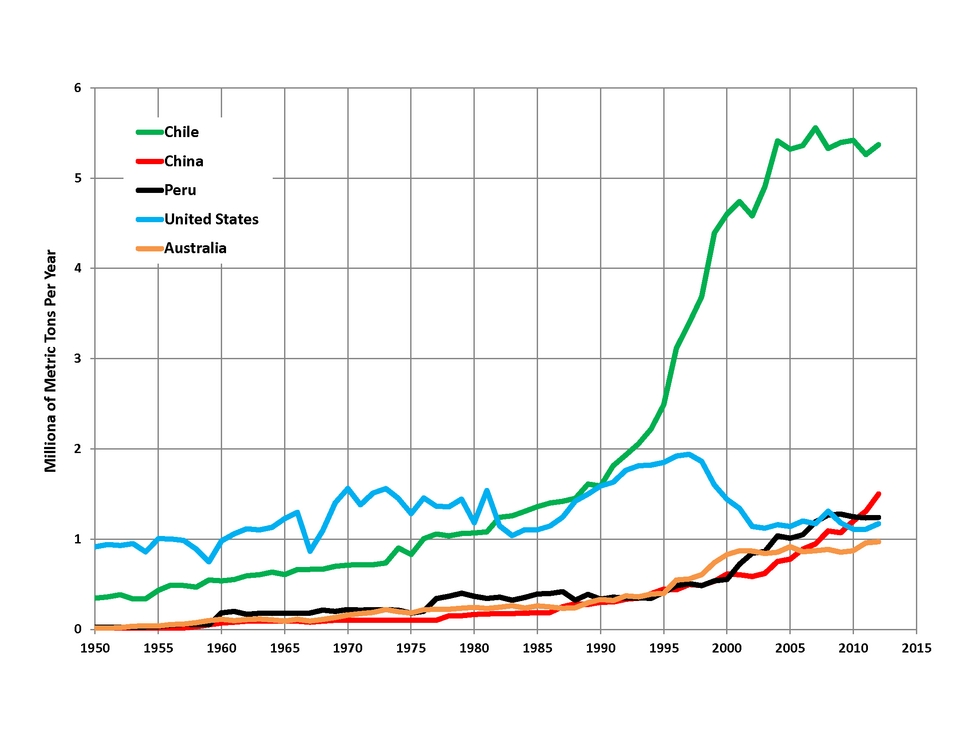
\includegraphics[width=0.5\linewidth]{Figures/image.png}
%     \caption{Wikipedia source}
%     \label{fig:placeholder}
% \end{figure}

% \vspace{1em}
% \vspace{1em}
% \subsection{Production Chain of Copper}

% The extraction of copper in Chile involves several key stages that transform low-grade ore into high-purity metal. It begins with \textbf{mining}, mainly through open-pit operations, where large quantities of rock containing less than 1\% copper are excavated. The ore is then crushed and processed in the \textbf{concentration} stage, where physical and chemical methods separate copper minerals to produce a concentrate containing about 25--35\% copper. This concentrate undergoes \textbf{smelting and refining}, where heat and chemical processes remove impurities, followed by \textbf{electrolysis} to achieve very high purity (up to 99.99\%). Finally, the refined copper is shaped during \textbf{final processing} into products such as wires, sheets, and alloys used in various industries. Together, these stages form a complex and resource-intensive process that is essential for supplying copper to global markets \cite{CNEP2025}.

% Copper mining in Chile is dominated by large-scale open-pit mines because many copper deposits are located close to the surface and extend over vast geographical areas. These mining operations require heavy machinery such as drills, excavators, loaders, and haul trucks to remove enormous quantities of waste rock and ore. In some cases, underground mining methods are also employed when ore bodies are located at greater depths. Once extracted, the ore is transported to nearby beneficiation plants where crushing and grinding operations reduce the material into fine particles to facilitate mineral separation.

% The concentration stage generally relies on flotation techniques, where chemical reagents and air bubbles are introduced into the crushed ore slurry to selectively separate copper-bearing minerals from waste material. The resulting copper concentrate contains significantly higher copper content and can then be economically transported to smelting facilities. Smelting represents one of the most energy-intensive stages of the production chain because the concentrate must be heated at extremely high temperatures to separate metallic copper from sulfur and other impurities. This process produces blister copper, which is then further purified during electrolytic refining to obtain cathode copper with purity levels suitable for industrial and electrical applications.

% In parallel to the traditional pyrometallurgical route, certain low-grade or oxide ores are processed using hydrometallurgical techniques such as \textbf{leaching-solvent extraction-electrowinning (LX-SX-EW)}. In this process, acidic solutions dissolve copper directly from the ore, after which solvent extraction purifies and concentrates the solution before electrowinning recovers pure copper metal. Compared to conventional smelting, this method generally requires lower temperatures and can be more suitable for specific ore types.

% The copper production chain also depends heavily on supporting infrastructure and industrial services. Transportation systems, electricity supply, water management facilities, tailings storage, and waste treatment operations are all necessary to maintain continuous production. Because many mining regions in Chile are located in arid areas such as the Atacama Desert, water supply and energy availability represent major operational challenges. Consequently, mining companies are increasingly investing in renewable energy systems, desalination plants, and more efficient technologies to reduce both operational costs and environmental impacts.

% Overall, the copper production chain combines highly advanced industrial processes with large-scale infrastructure and energy consumption. While these processes are essential for supplying global demand for copper, they also contribute significantly to greenhouse gas emissions and environmental pressures, making the modernization and decarbonization of the sector a major priority for Chile and the global mining industry.

% \cite{CNEP2025}.

% \subsection{Copper Extraction Process}

% The production of copper involves a sequence of interconnected industrial processes that transform raw ore into high-purity metal. These processes can be broadly divided into mining, beneficiation, smelting, refining, and hydrometallurgical treatment, each playing a critical role in the overall value chain.

% The process begins with \textbf{mining}, which can be performed using either open-pit or underground methods depending on the depth and geology of the ore deposit. Open-pit mining is the most common method, involving large-scale excavation of surface material in stepped benches, while underground mining uses shafts and tunnels to access deeper ore bodies. Both methods require heavy machinery and extensive infrastructure to extract and transport the ore to processing facilities.

% Once extracted, the ore undergoes \textbf{beneficiation}, also known as ore dressing or concentration. This stage involves crushing and grinding the ore into fine particles to liberate copper minerals from the surrounding rock. The material is then processed using flotation, a technique in which chemical reagents and air bubbles are introduced to selectively separate copper minerals. The result is a copper concentrate containing approximately 25--40\% copper, significantly increasing its economic value.

% The concentrated material is then sent to a \textbf{smelter}, where pyrometallurgical processes are used. In this high-temperature stage, the concentrate is heated in furnaces to remove impurities and separate metal from waste material (slag). This produces \textit{blister copper}, which typically contains around 98--99\% copper. Smelting is energy-intensive and contributes significantly to the overall emissions of the copper production chain.

% Following smelting, the copper undergoes \textbf{electrolytic refining}. In this process, copper anodes are dissolved in an electrolyte solution, and pure copper is deposited onto cathodes using an electric current. This electrochemical process removes remaining impurities and produces copper with a purity of up to 99.99\%, suitable for electrical and industrial applications.

% In parallel to the pyrometallurgical route, low-grade or oxide ores are often processed using a hydrometallurgical method known as \textbf{leaching-solvent extraction-electrowinning (LX-SX-EW)}. In this process, copper is first dissolved from the ore using acidic solutions (leaching). The solution is then purified and concentrated through solvent extraction (SX), and finally, copper is recovered as solid metal through electrowinning (EW). This method is particularly efficient for lower-grade ores and has lower energy requirements compared to traditional smelting.

% Finally, \textbf{production services} support all stages of copper extraction. These include material handling systems, transportation (trucks, conveyors), energy supply, water management, and waste treatment such as tailings storage. These supporting systems are essential for maintaining continuous and efficient operations throughout the entire process.

% In conclusion, copper production is a complex and resource-intensive process involving multiple stages that progressively increase the metal's purity and value. Both pyrometallurgical and hydrometallurgical routes are used depending on ore type, and modern operations rely heavily on advanced technologies and infrastructure to optimize efficiency and reduce environmental impact. 

% \subsection{Possible Main Drivers of CO$_2$ Emissions in Copper Extraction} 


% The main drivers of CO$_2$ emissions in copper extraction are associated with the high energy intensity and complexity of the production chain. A major source of emissions comes from \textbf{mining operations}, where diesel-powered machinery is used for drilling, blasting, and transporting large volumes of ore. Significant emissions also arise during \textbf{crushing and grinding} in the beneficiation stage, which require substantial electricity. The \textbf{smelting and refining} phases are particularly carbon-intensive due to the need for high-temperature furnaces, often powered by fossil fuels. In addition, \textbf{transportation} of ore, concentrate, and refined copper across long distances contributes to indirect emissions. The reliance on fossil-based energy for electricity generation further increases the overall carbon footprint. Finally, \textbf{waste management and tailings processing} can also contribute to emissions, especially when involving additional energy use and chemical treatments. Together, these factors make copper extraction a resource- and energy-intensive process with significant environmental impacts.

% \vspace{1em}


% \vspace{1em}
% \subsection{Copper as a Means to Reduce CO$_2$ Emissions}

% Copper is considered one of the most important strategic materials in the global transition toward a low-carbon economy because of its exceptional electrical and thermal conductivity. These physical properties make copper indispensable for the development, transmission, and efficient use of electricity in modern energy systems. As countries seek to reduce their dependence on fossil fuels and increase the share of renewable energy in their energy mix, the demand for copper continues to rise significantly. Renewable technologies such as solar photovoltaic panels, wind turbines, hydroelectric systems, and battery storage installations require substantially larger quantities of copper compared to conventional fossil-fuel-based technologies. This is mainly due to the need for efficient electrical connections, power conversion systems, generators, transformers, and transmission cables.

% Copper also plays a fundamental role in the electrification of transportation, which is considered one of the key solutions for reducing greenhouse gas emissions worldwide. Electric vehicles (EVs), including cars, buses, and rail systems, require considerably more copper than traditional internal combustion engine vehicles. Copper is extensively used in electric motors, batteries, inverters, charging stations, and onboard electrical systems because it enables efficient energy transfer and minimizes energy losses. In addition, the expansion of charging infrastructure and smart electricity grids further increases the importance of copper in supporting sustainable transportation systems. By facilitating the replacement of fossil-fuel-powered transport with electric alternatives, copper contributes directly to the reduction of CO$_2$ emissions associated with mobility and urban transportation.

% Beyond transportation and renewable electricity generation, copper is also essential for improving energy efficiency across industrial, residential, and commercial sectors. Efficient electrical systems reduce energy losses during transmission and distribution, thereby lowering the total amount of energy required for economic activities. Modern power grids, energy storage technologies, and advanced electronic systems all rely heavily on copper components to ensure reliable and efficient operation. Consequently, copper indirectly contributes to reducing global emissions by enhancing the overall efficiency of energy systems and enabling the integration of intermittent renewable energy sources into national electricity networks.

% Another major environmental advantage of copper lies in its recyclability. Copper can be recycled an unlimited number of times without losing its chemical or physical properties, making it highly suitable for circular economy strategies. Recycling copper requires significantly less energy than primary extraction and refining, which substantially reduces greenhouse gas emissions and decreases the environmental impact associated with mining activities. Secondary copper production therefore plays a crucial role in limiting the demand for newly mined copper while supporting sustainable resource management. Today, recycled copper already represents an important share of global copper production and is expected to become increasingly significant as demand for clean technologies continues to expand.

% Nevertheless, despite its positive contribution to decarbonization, copper production itself remains energy-intensive and can generate substantial CO$_2$ emissions. Mining operations, ore transportation, smelting, and refining processes often rely on fossil fuels and large amounts of electricity. This creates an important paradox in the energy transition: copper is essential for reducing emissions globally, yet its extraction and processing can contribute significantly to environmental pollution if not managed sustainably. For this reason, many countries, including Chile, are investing in cleaner mining technologies, renewable energy integration, and more efficient refining processes to reduce the carbon footprint of copper production.

% As global efforts to combat climate change intensify, copper is expected to remain at the center of decarbonization strategies. The growing deployment of renewable energy systems, electric vehicles, energy storage technologies, and electrified infrastructure will continue to increase copper demand in the coming decades. Consequently, ensuring a sustainable and low-carbon copper supply chain has become a critical challenge for governments, industries, and policymakers worldwide.


% \subsection{CO$_2$ Emissions Reduction in Chile}
% In 2020, Chile announced two targets for emissions reduction. The first, due in 2030, aims for an unconditional absolute target of 95~MtCO$_2$e or a cumulative emissions budget of 1{,}100~MtCO$_2$e, as well as a conditional emissions reduction target of up to 45\% net greenhouse gas (GHG) emissions reduction, subject to specific financial, market, technological, and political conditions \cite{CATChile2020}.

% Chile has made significant progress in reducing CO2 emissions through various initiatives and policies in the past few years.  

% \begin{figure}[H]
%     \centering
%     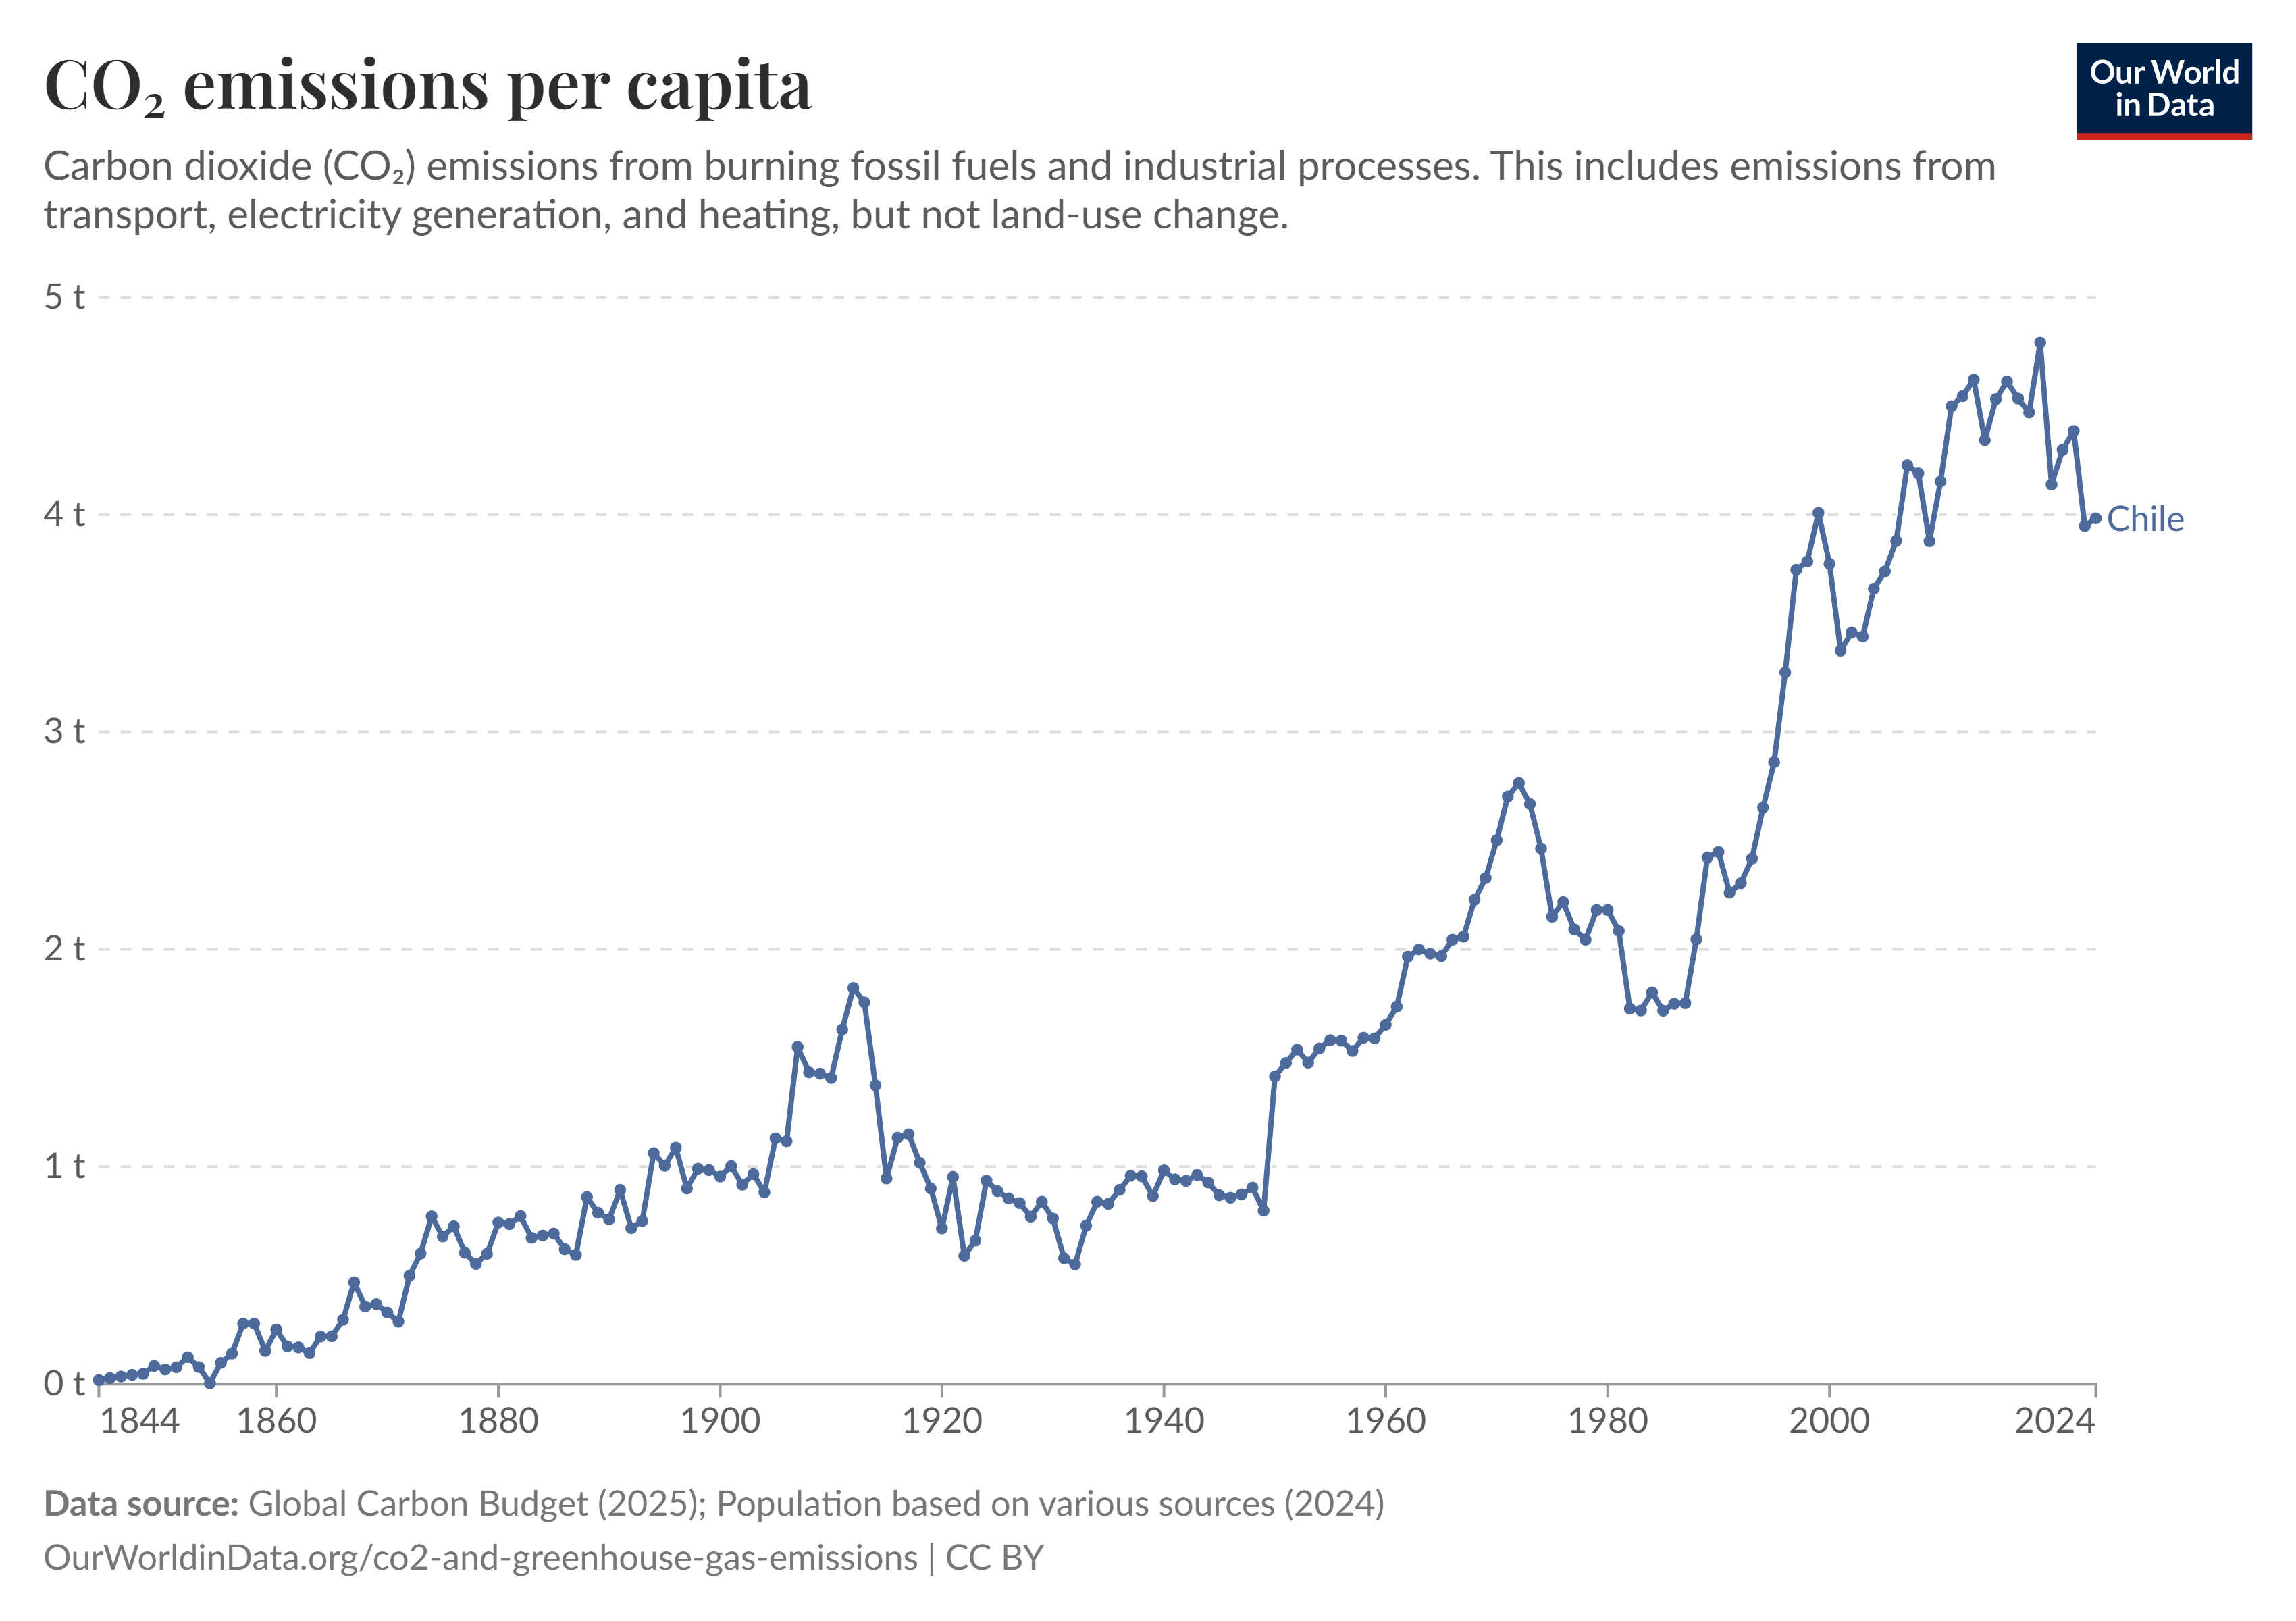
\includegraphics[width=0.5\linewidth]{Figures/co-emissions-per-capita (1).png}
%     \caption{Enter Caption}
%     \label{fig:placeholder}
% \end{figure}



% https://greeniron.se/visit-in-chile-one-of-the-worlds-leading-mining-countries/?
% \vspace{1em}
% Global Journal of Flexible Systems Management (December 2025) 26(4):813–837
% https://doi.org/10.1007/s40171-025-00464-w
    \newpage

\section{Existing Studies on Copper Mining and CO$_2$ Emissions}
	\subsection{Contribution of Copper Mining to Global Emissions}

Copper plays a central role in the global energy transition due to its extensive use in renewable energy systems, electric vehicles, electricity grids, and energy storage technologies. According to the International Energy Agency (IEA), electric vehicles require approximately 2.5 times more copper than conventional internal combustion vehicles \cite{IEA2021}. As a result, several studies project a significant increase in copper demand under global decarbonization scenarios \cite{Watari2020}. The IEA estimates that copper demand from clean energy technologies alone could more than double by 2040 under a net-zero emissions pathway \cite{IEA2021}.

At the same time, copper extraction and processing remain highly energy-intensive activities requiring large quantities of fuel and electricity \cite{Norgate2010}. Chile currently accounts for more than 25\% of global copper production, making the environmental performance of its mining sector particularly important at the global scale \cite{CochilcoWebsite2025}. Consequently, a growing body of literature focuses on the environmental sustainability of copper supply chains and the challenge of reducing emissions associated with mining and mineral processing activities \cite{Elshkaki2018}.


\subsection{Historical Evolution of Mining Energy Consumption}
\label{sec:evol of mining energy}

Several studies have examined the historical evolution of energy consumption in metallic mining and its relationship with industrial development \cite{Norgate2010,Northey2014}. In copper mining, energy demand has increased steadily over recent decades alongside the expansion and increasing complexity of mining operations.

Mining energy consumption is generally divided into direct and indirect components. Direct energy consumption mainly corresponds to fuel combustion in trucks, excavation equipment, and transportation systems, while indirect energy consumption refers to electricity use in crushing, grinding, concentration, pumping, and refining processes. Existing studies emphasize that electricity consumption has become increasingly important in modern copper mining because mineral processing operations are highly electricity-intensive \cite{Norgate2010}. For example, concentrator plants in Chile consume more than 10,000 MJ of electricity per tonne of copper concentrate produced \cite{Cochilco2024}.

The literature also highlights that technological improvements and process optimization have partially reduced energy requirements in certain mining activities. However, total energy consumption in the sector has generally continued to increase due to the scale and growing complexity of production systems \cite{Calvo2016}.


\subsection{Ore Grade Decline and Energy Demand}

Declining ore grades are widely recognized as one of the main structural challenges facing the mining industry \cite{Calvo2016,Northey2014}. Ore grade refers to the concentration of valuable metal contained in the extracted rock. As ore grades decline, larger quantities of material must be extracted and processed in order to produce the same quantity of refined copper.

Several studies identify ore grade decline as a major driver of increasing energy consumption in copper mining \cite{Calvo2016}. Lower ore concentrations require additional crushing, grinding, concentration, and waste management operations, all of which increase energy requirements throughout the production chain. Northey et al. show that average copper ore grades in many mining operations have fallen below 1\% over recent decades \cite{Northey2014}. In Chile, average ore grades in concentrator plants declined from approximately 0.87\% in 2015 to around 0.66\% in 2024 \cite{Cochilco2024}.

Because ore grade is determined by geological conditions and resource depletion, this trend represents a long-term structural constraint that may progressively increase the energy requirements associated with copper production.


\subsection{Electrification and Renewable Integration}
\label{sec:elec & renew}
In response to growing environmental concerns, many studies explore potential decarbonization pathways for the mining industry. Electrification of mining equipment and integration of renewable electricity are among the most frequently proposed strategies for reducing greenhouse gas emissions in copper production \cite{Memary2022}. Existing research suggests that replacing diesel-powered systems with electric technologies could reduce direct emissions from mining operations, while decarbonizing electricity generation could lower indirect emissions associated with electricity-intensive mineral processing.

Several studies identify Chile as particularly well positioned for this transition because of its exceptional renewable energy potential, especially solar energy in the Atacama Desert and wind energy in coastal regions \cite{IEAChile2026}. Renewable sources represented nearly 70\% of Chile’s electricity generation in 2024, while wind and solar energy alone exceeded 40\% of monthly electricity generation for the first time in December 2024 \cite{EnergiaEstrategica2025,Ember2025}.

The literature nevertheless emphasizes that reducing emissions from copper mining will likely require a combination of renewable electricity integration, technological innovation, process efficiency improvements, and broader industrial decarbonization strategies \cite{Memary2022}.


\subsection{Methodologies for Emissions Decomposition}

Several methodological approaches have been developed to analyse greenhouse gas emissions in industrial sectors, including decomposition methods such as the Kaya identity, IPAT frameworks, and Logarithmic Mean Divisia Index (LMDI) techniques. These approaches are widely used to separate the influence of activity growth, energy intensity, and carbon intensity on total emissions \cite{Tilton1998,Norgate2010}.

In the context of copper mining, decomposition methods are particularly relevant because emissions are influenced simultaneously by production growth, ore quality, energy consumption, and the carbon intensity of fuel and electricity use. These interacting drivers motivate the use of an IPAT-based framework capable of separating geological, technological, and energy-related contributions to CO$_2$ emissions.


    \newpage

\section{Possible Main Drivers of CO$_2$ Emissions in Copper Production}
    Copper production emissions are influenced by several interacting geological, technological, and energy-related factors. The complexity of the copper production chain implies that greenhouse gas emissions cannot be attributed to a single source alone. Instead, emissions result from the combined effects of production growth, ore quality, energy consumption, process characteristics, and the carbon intensity of the energy system. Understanding these different drivers is therefore essential for identifying potential technological and policy levers capable of reducing the environmental impact of copper mining.


\subsection{Production Growth}

One of the most direct drivers of CO$_2$ emissions is the total quantity of copper produced. As global demand for copper increases due to electrification and renewable energy deployment, mining operations must extract and process larger quantities of ore. The International Energy Agency projects that copper demand from clean energy technologies alone could more than double by 2040 under global net-zero scenarios \cite{IEA2021}. Higher production volumes generally require additional energy consumption across all stages of the production chain, including extraction, transportation, concentration, smelting, and refining processes. Consequently, production growth tends to increase both direct and indirect greenhouse gas emissions.

\subsection{Ore Grade Decline}

Ore grade represents the concentration of copper contained in extracted rock and constitutes one of the main structural constraints affecting mining sustainability. As ore grades decline, larger quantities of material must be extracted, transported, crushed, and processed in order to produce the same quantity of refined copper. Several studies report a long-term decline in average copper ore grades worldwide, with many operations now exploiting ores below 1\% copper concentration \cite{Northey2014,Calvo2016}. In Chile, average ore grades in concentrator plants declined from approximately 0.87\% in 2015 to around 0.66\% in 2024 \cite{Cochilco2024}. This increases energy requirements throughout the production chain and contributes directly to higher greenhouse gas emissions.

Unlike technological variables, ore grade is largely determined by geological conditions and resource depletion. Consequently, declining ore grades create a long-term structural pressure on mining energy consumption that may partially offset efficiency improvements achieved through technological progress.


\subsection{Energy Intensity of Mining Processes}

Copper production is highly energy-intensive due to the scale and complexity of mining and mineral processing operations. Different stages of the production chain require different forms and quantities of energy. Mining and transportation activities mainly rely on diesel-powered machinery, while crushing, grinding, concentration, electro-winning, and refining processes consume large amounts of electricity.

Existing studies show that concentrator plants are among the most energy-intensive stages of copper production. Cochilco reports electricity consumption levels exceeding 10,000 MJ per tonne of concentrate produced in certain concentration processes \cite{Cochilco2024}. At the national level, total energy consumption associated with Chilean copper mining increased by more than 15\% between 2015 and 2024 despite relatively stable production volumes. Energy intensity therefore constitutes a major determinant of CO$_2$ emissions.


\subsection{Electrification and Electricity Carbon Intensity}
\label{sec:elec and CI}
The distinction between direct and indirect emissions is particularly important in copper production. Direct emissions mainly originate from fuel combustion in extraction and transportation equipment, while indirect emissions are associated with electricity generation used throughout mineral processing operations.

Indirect emissions historically represented the largest share of emissions in Chilean copper mining due to the high electricity requirements of concentration and refining processes \cite{CochilcoEmissions2024}. However, the rapid decarbonization of Chile’s electricity system has significantly reduced the carbon intensity of electricity generation over recent years. Renewable sources represented nearly 70\% of Chile’s electricity generation in 2024 \cite{EnergiaEstrategica2025}. As a result, indirect emissions associated with electricity use in copper mining have declined substantially over the last decade.

Electrification of mining equipment is increasingly considered a major decarbonization pathway for the mining industry. However, the environmental benefits of electrification depend strongly on the carbon intensity of the electricity system. Consequently, future emissions reductions will depend both on technological changes within mining operations and on the continued decarbonization of electricity generation.


\subsection{Process Heterogeneity Along the Production Chain}
\label{sec:heterogeneity}
The different stages of copper production contribute unevenly to total energy consumption and greenhouse gas emissions. Certain operations, such as grinding, concentration, and smelting, are particularly energy-intensive, while others contribute comparatively less to total emissions. Moreover, the relative importance of fuel and electricity differs significantly between processes.

For example, mining and transportation stages rely predominantly on fuel combustion, whereas concentration and electro-winning processes are largely electricity-intensive \cite{Cochilco2024}. Understanding the heterogeneity of emissions across the production chain is therefore essential for identifying the most effective decarbonization strategies. Reducing emissions in processes with high energy consumption may have a significantly larger impact on total emissions than improving smaller contributors. Consequently, analysing the contribution of each process separately provides a more precise understanding of the technological and energy-related drivers influencing copper production emissions.
    \newpage
    
\section{Regulatory Framework and Decarbonization Policies}
    
\subsection{Global Climate Commitments and Critical Minerals}
\label{sec:global climate commitments}
The global transition toward a low-carbon economy has significantly increased the strategic importance of critical minerals such as copper. International climate objectives established under the Paris Agreement require a rapid deployment of renewable energy systems, electric vehicles, electricity grids, and energy storage technologies, all of which depend heavily on copper-intensive infrastructure. As a result, several governments and international organizations have developed policies aimed at securing the long-term supply of critical minerals while reducing the environmental impact associated with their extraction and processing.

In parallel, many countries have adopted net-zero emissions targets and industrial decarbonization strategies. These policies increasingly emphasize the need to reduce greenhouse gas emissions across mineral supply chains while ensuring sufficient availability of raw materials required for the energy transition.


\subsection{Chilean Climate and Energy Policies}

Chile has established ambitious climate objectives aimed at supporting the global energy transition while reducing greenhouse gas emissions from its energy-intensive industries. Through its updated Nationally Determined Contribution (NDC) and Climate Change Framework Law, Chile has committed to achieving carbon neutrality by 2050 \cite{CAT2020}. The country also plans to progressively phase out coal-fired electricity generation and accelerate the expansion of renewable energy production.

Chile occupies a particularly favorable position in this transition because of its exceptional renewable energy potential, especially solar energy in the Atacama Desert and wind energy in coastal regions \cite{SolarAtlas2019}. Renewable sources represented nearly 70\% of Chile’s electricity generation in 2024 \cite{EnergiaEstrategica2025}. These developments are particularly important for the mining sector because electricity generation strongly influences the indirect emissions associated with copper extraction and mineral processing.


\subsection{Sustainability Standards in the Mining Sector}

Several international organizations and industry initiatives promote sustainability and emissions reduction in the mining sector. The International Council on Mining and Metals (ICMM) establishes environmental and climate-related principles for mining companies, including commitments related to emissions reduction, responsible resource management, and transparency. Similarly, the International Copper Association (ICA) supports research and sustainability initiatives related to copper production and lifecycle management.

More recently, certification frameworks such as the Copper Mark have emerged to encourage compliance with environmental, social, and governance (ESG) standards across the copper value chain. These initiatives aim to improve transparency, strengthen environmental accountability, and promote more sustainable mining practices through independent verification processes.


\subsection{Decarbonization Challenges for Copper Mining}

Despite the rapid expansion of renewable electricity and increasing sustainability commitments, several studies emphasize that decarbonizing copper mining remains a major industrial challenge. Copper demand is expected to increase significantly under global electrification scenarios, while declining ore grades and increasing extraction complexity continue to raise energy requirements in mining operations.

Consequently, future emissions reductions in the copper sector will likely depend on a combination of renewable electricity integration, electrification of mining equipment, improvements in process efficiency, and technological innovation. These interacting technological and structural constraints motivate the need for decomposition approaches capable of separating the different drivers influencing CO$_2$ emissions in copper mining.

\subsection{Relation Between Copper Production Decarbonization and Sustainable Development Goals}

While the United Nations Sustainable Development Goals (SDGs) were not specifically designed for the mining sector, copper production and its decarbonization are closely connected to several of these global objectives. As copper is an essential material for renewable energy systems, electric vehicles, electricity grids, and energy storage technologies, the sector plays a major role in supporting the global energy transition.

The transition toward lower-emission copper production aligns particularly well with the following SDGs:

\begin{itemize}
    \item \textbf{SDG 7 -- Affordable and Clean Energy:} promotes the expansion of renewable electricity generation and electrification technologies, both of which rely heavily on copper-intensive infrastructure.

    \item \textbf{SDG 9 -- Industry, Innovation and Infrastructure:} encourages the development of more sustainable industrial systems through technological innovation, process efficiency improvements, and cleaner mining operations.

    \item \textbf{SDG 12 -- Responsible Consumption and Production:} supports more sustainable resource management practices, including emissions reduction, energy efficiency, and recycling within the copper value chain.

    \item \textbf{SDG 13 -- Climate Action:} calls for urgent measures to reduce greenhouse gas emissions and mitigate climate change, objectives that are directly related to the decarbonization of mining activities.
\end{itemize}
    \newpage
    
\section{Decomposition analysis}
\label{sec:decomposition}
    \subsection{Kaya Decomposition}

To understand the emissions of CO\textsubscript{2} of copper production Chili we need to decompose in more granular components in order to identify the technological and policy levers available to reduce CO\textsubscript{2} emissions from Chilean copper production. The decomposition is the following: 

\begin{equation}
\text{CO}_2 = \text{Ore} \times \frac{\text{prod}}{\text{Ore}} \times \frac{E_{\text{tot}}}{\text{prod}} \times \sum_{i} \left[ \frac{E_i}{E_{\text{tot}}} \times \left( \frac{E_{\text{comb},i}}{E_i} \cdot \text{CI}_{\text{comb,i}} + \frac{E_{\text{elec},i}}{E_i} \cdot \text{CI}_{\text{elec,i}} \right) \right]
\end{equation}

where $i \in \{\text{Open pit, Underground mining, Concentrating plant, Smelter, Electrolytic refining,}$\\
$\text{LX-SX-EW, Services}\}$
\\
To have a global view of the environmental impact the production cycle of copper we decided to look at the impact of each process along production chain. The sum over i decomposes the impact for every processes.
\\
\textbf{Production and ore processing:}
\begin{itemize}
    \item $\text{Ore}$ = Quantity of ore mined [kT], calculated as $\text{Ore} = \frac{\text{prod}}{\text{grade}}$
    \item $\text{prod}$ = Total copper production (cobre fino) [kT]
    \item $\frac{\text{prod}}{\text{Ore}}$ = Average Chilean ore grade [\%]
\end{itemize}

\textbf{Energy consumption:}
\begin{itemize}
    \item $\frac{E_{\text{tot}}}{\text{prod}}$ = Total energy intensity across all processes [MJ/kT copper]
    \item $\frac{E_i}{E_{\text{tot}}}$ = Share of total energy consumed by process $i$
    \item $E_{\text{tot}} = \sum_{i} E_i$ = Total energy consumption [MJ]
\end{itemize}

\textbf{Energy mix by process:}
\begin{itemize}
    \item $\frac{E_{\text{comb},i}}{E_i}$ = Fraction of combustion fuel energy in process $i$
    \item $\frac{E_{\text{elec},i}}{E_i}$ = Fraction of electricity in process $i$
    \item $E_i = E_{\text{comb},i} + E_{\text{elec},i}$ for each process $i$
\end{itemize}

\textbf{Carbon intensity:}
\begin{itemize}
    \item $\text{CI}_{\text{comb,i}} = \frac{\text{CO}_{2,\text{comb,i}}}{E_{\text{comb,i}}}$ = Carbon intensity of combustion fuels (direct emissions) in process $i$ [kT CO\textsubscript{2}/MJ]
    \item $\text{CI}_{\text{elec,i}} = \frac{\text{CO}_{2,\text{elec,i}}}{E_{\text{elec,i}}}$ = Carbon intensity of electricity (indirect emissions) in process $i$ [kT CO\textsubscript{2}/MJ]
\end{itemize}

Each ratio highlights a possible lever of action to reduce CO\textsubscript{2}, it can be a technological lever or a policy lever. At the same time we can analyze which are the main drivers of greenhouse emission due to copper production in Chili.
\subsection{Interpretation of components}
\textbf{Ore grade} is an important driver of impact because the density of copper in the ground varies and diminishes the deeper the mine is. It requires more energy and work, therefore more ore extracted, to get the same amount of copper produced. Ore grade has a direct impact on emissions. Moreover, ore grade is a variable that is not manageable by humans; it is a natural constraint that we will face by extracting more and more copper. Thus, it is very important to act on other levers to diminish the impact.
\\\\
\textbf{Total energy intensity} gives an important overview of how energy intensity evolved over the years. It doesn't give precise information about which process has the most impact or how their energy intensity changed, but it provides an overview of how the copper production chain's energy intensity has progressed.
\\\\
\textbf{Carbon intensity type by process} is very important to dig deeper into the decomposition and have a clearer and more precise view of which processes and which source of energy (either direct from fuel or indirect from electricity) are the most carbon intensive and where there is the most space for improvement. For carbon intensity from direct emissions, it is a good proxy of technological development, whether the machines and techniques used during the production process are more efficient and less polluting for the same energy consumption. On the other hand, for the use of indirect energy, the carbon intensity is also a good proxy to know how electricity is produced and what the principal sources are, whether they are renewable or not.
\\\\
\textbf{Fraction of energy type by process} is a crucial component of our decomposition and a lever to decarbonize the sector. As discussed in the paragraph above, technological improvement can have a great impact on carbon intensity for direct emissions; however, we can also see technological improvement as a shift from fuel usage to electricity. It is important to keep in mind that this shift is meaningful only if electricity production in Chile is also evolving toward sustainable production from renewable sources. We will discuss this in more detail later on.
\\\\
\textbf{Share of total energy by process} is a meaningful component because it gives a clear view of the importance of each process in the copper production cycle. Working on the emissions of the biggest processes is a much bigger lever on the impact due to their energy consumption. If the carbon intensity of a low energy consumption process is diminished, it would be much less impactful on emissions than improving a process with a high share of total energy consumption. Thus, it is very important to focus on the right processes.
\subsection{Components to TAP}
In the previous subsection, we have already given a first hint of how the components of the decomposition could be associated with technology, affluence, and population. Even though there is no population in this decomposition, the ore serves as it, because it represents all the rock extracted from the ground. Affluence in this decomposition represents the level of copper density in the ground, in other words, ore grade. The rest of the decomposition can be associated with technology. Since it is a Kaya decomposition, "technology" is broken down into two parts: energy intensity and carbon intensity. Furthermore, the decomposition breaks down carbon intensity by another level by looking at each process and at the source of energy, either direct (fuel) or indirect (electricity).
\subsection{Data Sources}
The data used to analyse this decomposition relies on one main source. The dataset used is published by COCHILCO (COMISIÓN CHILENA DEL COBRE), which is the Chilean commission of copper. The main mission of COCHILCO is to oversight the copper industry and advice the government so that this sector is preserved and can continue to develop in sustainable way.\cite{CochilcoWebsite2025} The Excel file with the data used and plenty of other data can be found on there website under publications (publicaciones) and then under sustainability (sustentabilidad). The dataset used goes from 2015 to 2024. \footnote{https://www.cochilco.cl/web/\#}
\subsection{Evolution of CO$_2$ drivers in copper production}

\begin{figure}[H]
    \centering
    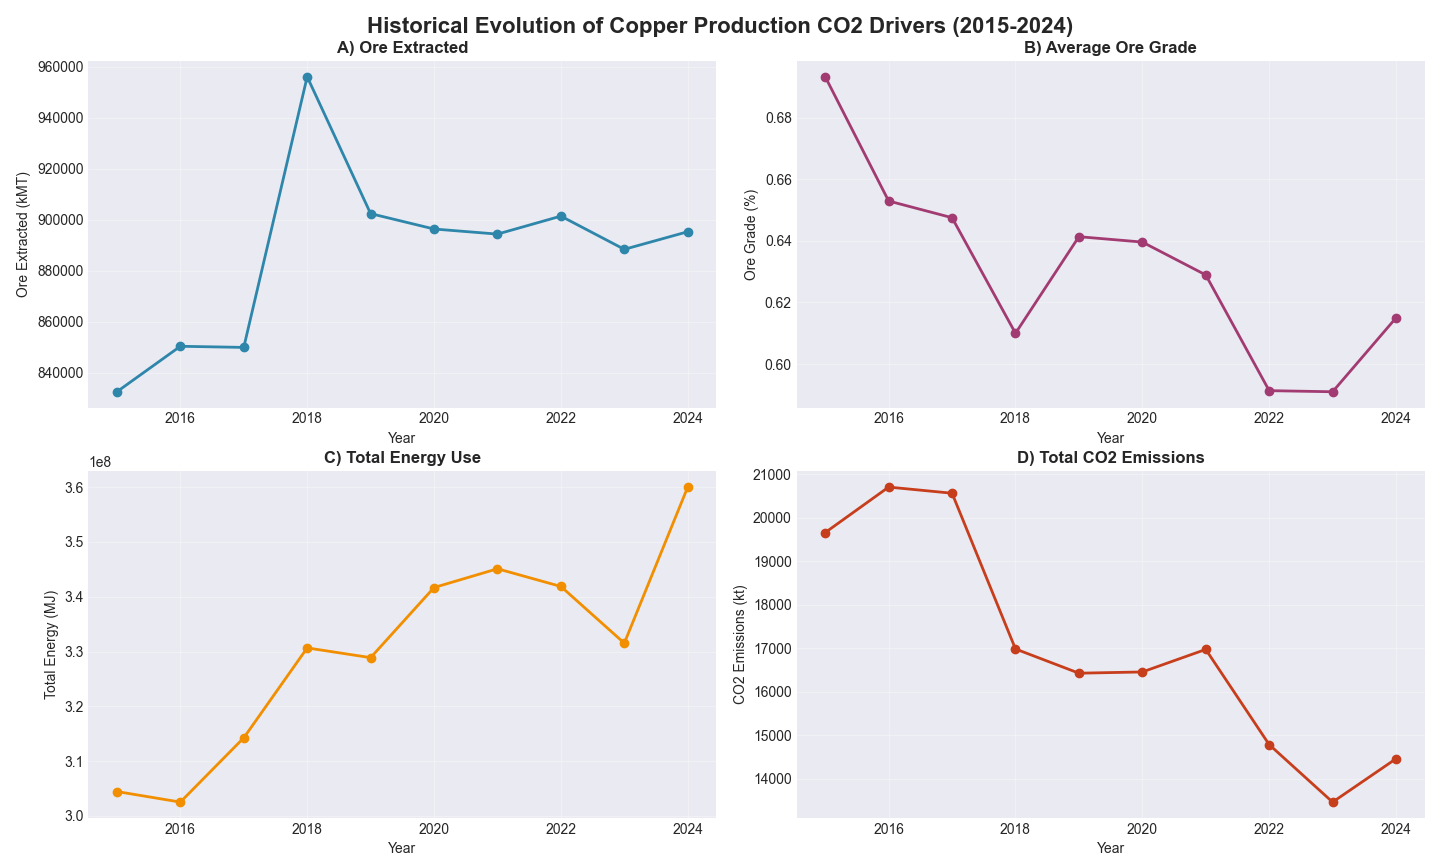
\includegraphics[width=0.9\linewidth]{Figures/Figure_1.png}
    \caption{Historical Evolution of Copper Production CO2 Drivers (2015-2024)}
    \label{fig:cen_region}
\end{figure}
\textbf{Panel A:} shows the evolution of ore extracted in metric tonnes. Between 2017 and 2018 we see a very high increase but then on a stabilization around 900'000 kT. 
\\\\
\textbf{Panel B:} highlights how the average ore grade of copper evolved over the years. We can clearly see a downward trend with a decrease higher than 10\% over ten years. Years where ore grade improved (2019 and 2024) were probably due to the discovery of new reserves with higher copper concentration in the ground.
\\\\
\textbf{Panel C:} displays how total energy consumption during the production cycle evolved between 2015 and 2024. The upward trend is clear, with more than a 15\% increase in energy consumption. This increase can clearly be associated with the decrease in ore grade, which translates into much more rock extraction from the ground. Between 2020 and 2022, energy consumption stabilized during years when production also decreased, suggesting a direct link between production volume and energy use.
\\\\
\textbf{Panel D:} tracks the total amount of greenhouse gas emissions due to copper production. Over the years, there has been a constant downward trend with a decrease of one third. While energy consumption increased, this suggests that important improvements have been made to limit CO$_2$ emissions over the last ten years. 
\\\\
These four figures highlight that the amount of ore extracted has been quite constant over years (apart from a peak in 2018), while ore grade clearly had a downward trend and energy consumption an upward trend. Because ore extracted has been quite constant in the previous year while ore grade declined, it suggests that production of copper has also a bit declined. The most important point is to see that overall, the total amount of CO$_2$ emissions has decreased by more than 20\%, showing that progress has been made and can continue to be made. In the next sections, we will try to dig deeper and explore in more detail what are the causes and reasons for this decline and what can still be done to reduce the impact of copper production in Chile. As discussed in section \ref{sec:evol of mining energy}, the scale and growing complexity of production has increased the total energy consumption.
\subsection{Carbon Intensity and Electrification Indicators}
\begin{figure}[H]
    \centering
    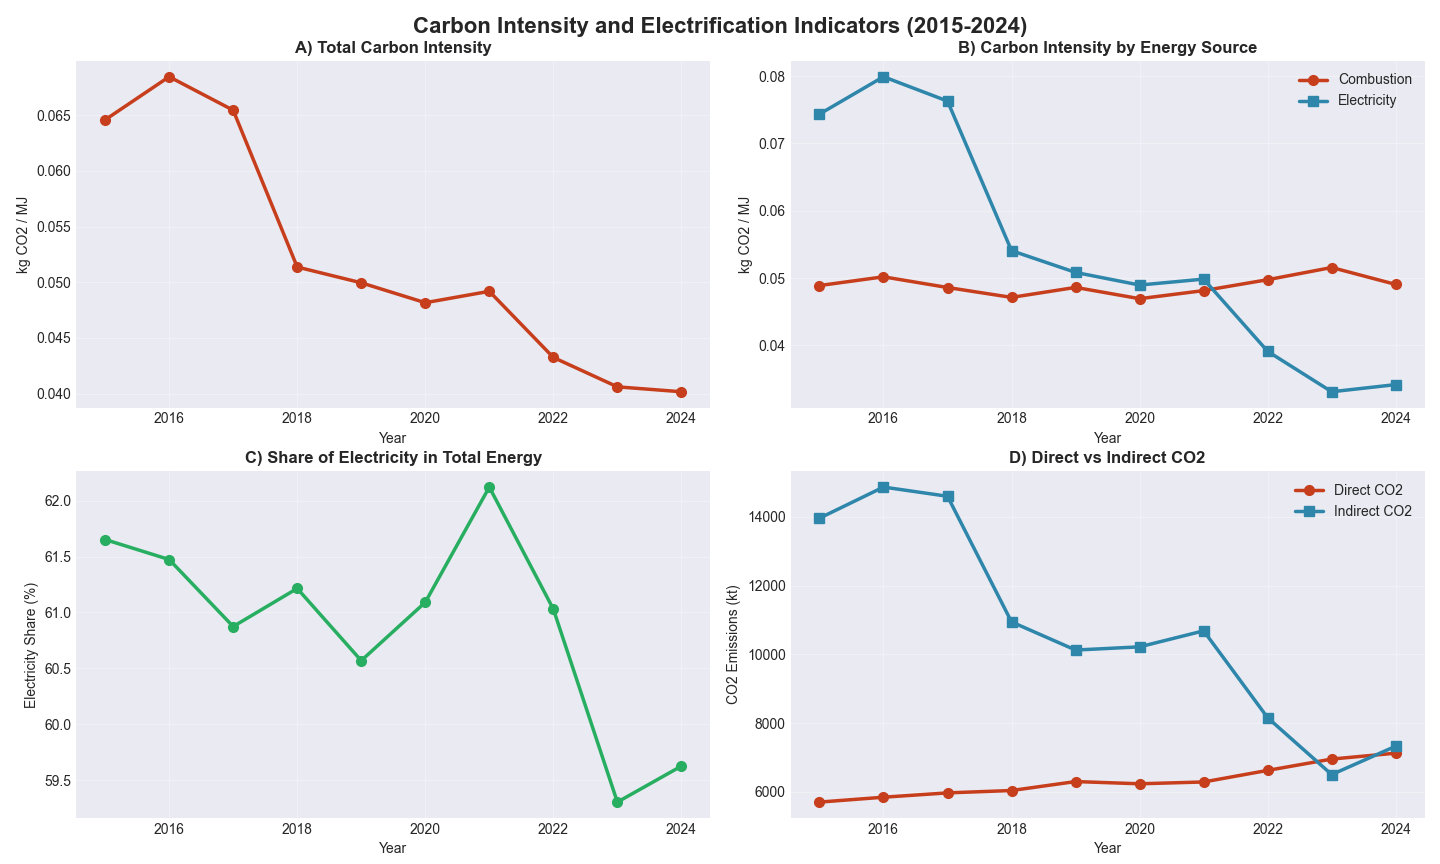
\includegraphics[width=0.9\linewidth]{Figures/Figure_2.png}
    \caption{Carbon Intensity and Electrification Indicators (2015-2024)}
    \label{fig:cen_region}
\end{figure}
\textbf{Panel A:} shows how carbon intensity evolved over the years. In this case, it is the total carbon intensity and it is not decomposed between direct and indirect carbon intensity. Over the years, there is a downward trend, with a total decrease of around one-third.
\\\\
\textbf{Panel B:} compares the evolution of carbon intensity from direct use of energy (fuel) and indirect use of energy (electricity). The carbon intensity from direct emissions stays constant over the years, while the carbon intensity from electricity has decreased by half over the last ten years. This suggests that overall, machines or processes using fuel have not evolved much in terms of efficiency, while the production of electricity used in copper production has diminished its impact considerably.
\\\\
\textbf{Panel C:} displays the evolution of the electricity share in energy use. There has been a small downward trend between 2021 and 2024, but overall the share of electricity remained constant at around 61\%.
\\\\
\textbf{Panel D:} highlights the variation of direct and indirect CO$_2$ emissions. Direct emissions increased by approximately 10\%, while indirect emissions decreased by more than 50\%. Indirect emissions used to be the largest driver of total emissions, this is consistent with what has been discussed and highlighted in section \ref{sec:elec and CI}. This suggests that the decrease over the years in greenhouse gas emissions is mostly due to the decrease in emissions coming from electricity use. 
\\\\
These four figures highlight how the reduction in carbon intensity of electricity production in Chile has helped to decrease emissions in the copper production chain toward more sustainable sources. They also suggest that in terms of technical evolution of machines using fuel, overall their emissions didn't improve since the carbon intensity remained quite constant. On the other hand, the electricity share didn't evolve much either, strongly suggesting that the decrease in CO$_2$ is probably mainly due to the improvement of carbon intensity in electricity production. This highlights that Chile's renewable energy transition has been the primary driver of emissions reduction in the copper sector, rather than improvements in mining technology itself. We will explore the carbon intensity (direct and indirect) of the different processes and look at which have possible improvements and how they evolved over the years.
\subsection{Identify Key Drivers of CO2}
\begin{figure}[h]
    \centering

    \begin{subfigure}{0.7\textwidth}
        \centering
        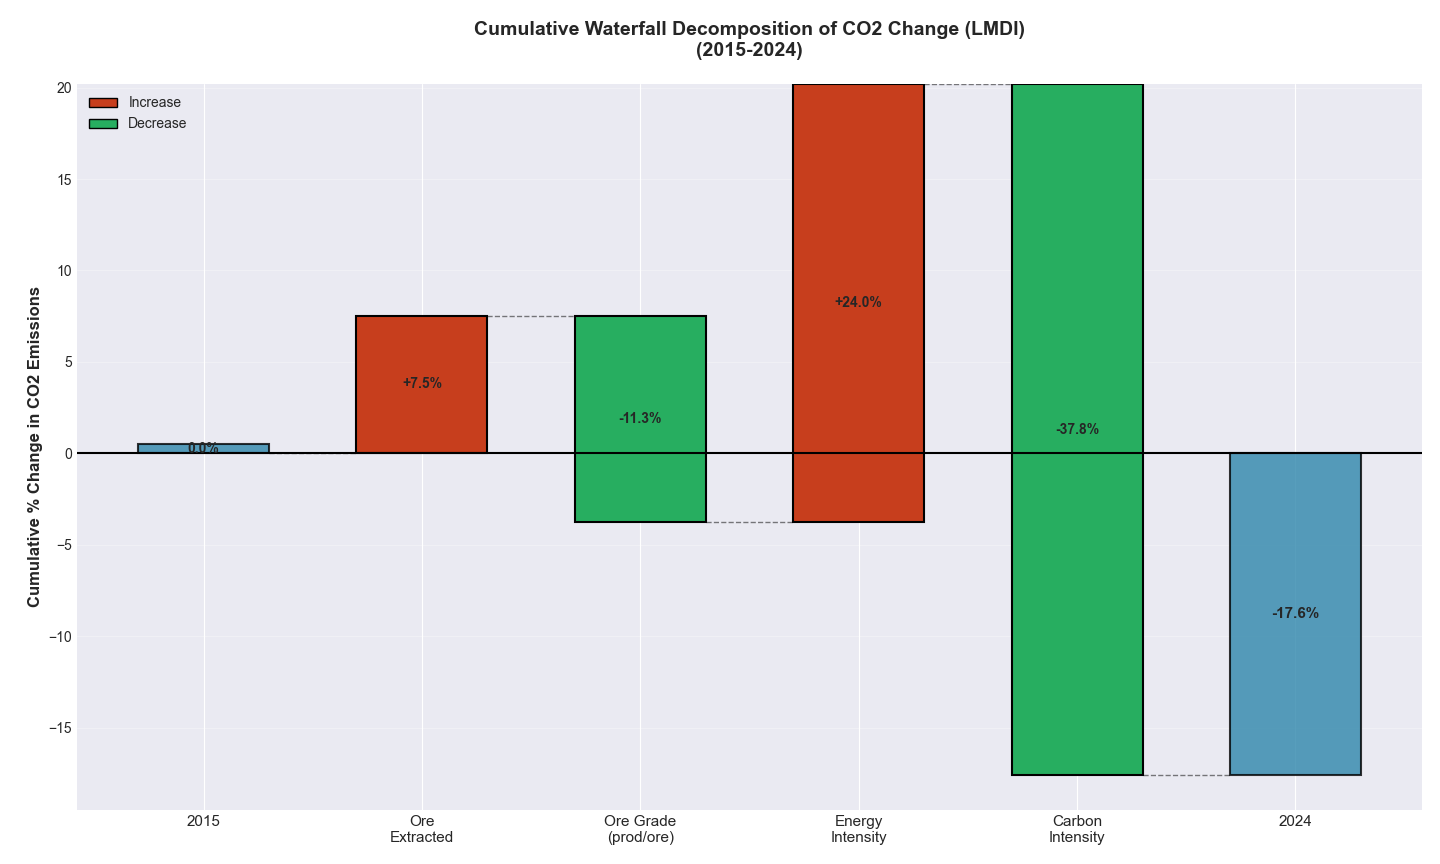
\includegraphics[width=\linewidth]{Figures/Figure_3.png}
        \caption{Cumulative Waterfall Decomposition of CO2 (LMDI)}
    \end{subfigure}
    \begin{subfigure}{0.7\textwidth}
        \centering
        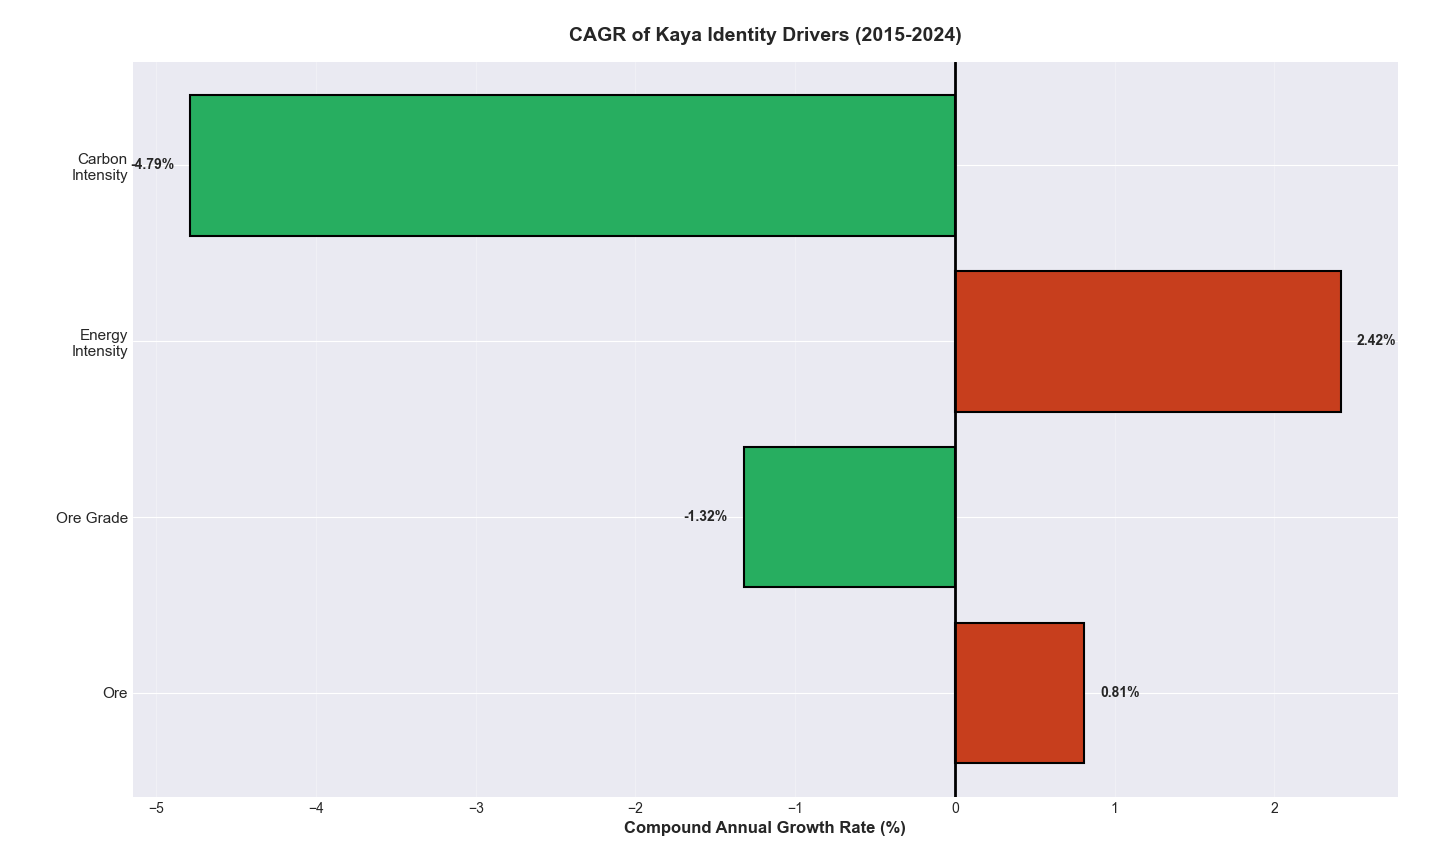
\includegraphics[width=\linewidth]{Figures/Figure_5.png}
        \caption{CGAR of Kaya Identity Drivers}
    \end{subfigure}
\end{figure}
\label{fig:waterfall}
The first figure is a waterfall chart that distributes the change in CO$_2$ emissions from copper production across the four components of the Kaya Identity using the LMDI method, while the second figure shows the compounded growth rate of the different Kaya Identity drivers. In the Kaya decomposition introduced earlier, carbon intensity corresponds to the aggregate contribution of all processes.

The combined effect of the growth in ore extraction and the decline in ore grade equals the growth rate in copper production between 2015 and 2024 (\textbf{7.5\% - 11.3\% = -3.8\%}), indicating that copper production declined over the period. This suggests that, although the quantity of ore extracted increased, it was not sufficient to offset the sharp decline in ore grade, resulting in a negative contribution to CO$_2$ emissions. This is also visible in the second figure, where the compounded growth rate of ore grade outpaces the growth rate of ore extraction.

Although energy intensity increased by \textbf{24\%}, total greenhouse gas emissions decreased over the years. This represents an absolute decoupling, driven primarily by the \textbf{37.8\%} reduction in carbon intensity. This is also visible in the CAGR graph, where the decline in carbon intensity (\textbf{-4.79\%}) outweighs the increase in energy intensity (\textbf{2.42\%}). These two charts therefore confirm the previous discussion: grid decarbonization was the main factor behind the decline in CO$_2$ emissions.


\subsection{Energy intensity and energy mix by process}
\begin{figure}[H]
    \centering
    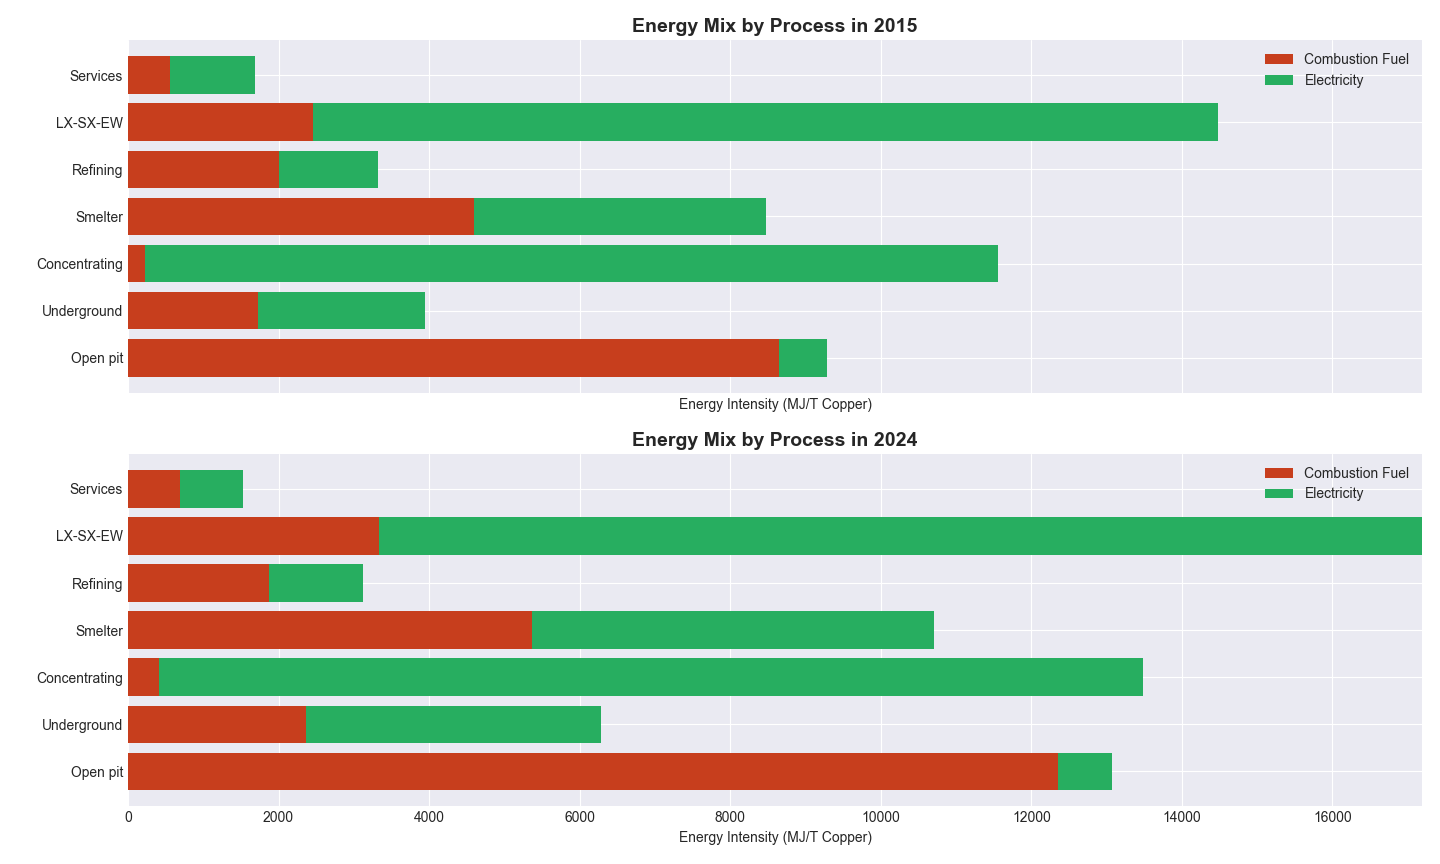
\includegraphics[width=1\linewidth]{Figures/Figure_4.png}
    \caption{Energy intensity and energy mix by process by process)}
    \label{fig:cen_region}
\end{figure}
This graph shows the total energy intensity, as well as its decomposition into direct and indirect energy intensity for each process in 2015 and 2024. We can clearly see that the activities related to the mining of copper (open pit and underground) are the most energy intensive and consume the most fuel energy. This suggests that much of the mining, especially open pit mining, is done with fuel combustion machines. LX-SX-EW is the second most energy intensive process, with a very large portion coming from electricity use due to electrowinning, where electric current drives the reduction of copper ions to metal. This once again demonstrates the importance of grid decarbonization. Apart from services and refining, every process increased its energy intensity, which is consistent with the increase in energy intensity seen in Figure \ref{fig:waterfall}.
\\
We can also remark that the share of electricity seems to stay approximately constant over the period, which suggests once again that the decrease in carbon intensity and therefore in greenhouse gas emissions is mainly due to grid decarbonization. We can also note that the overall electricity share of only \textbf{60\%} is mainly due to the open-pit mining process. Excluding open-pit mining, the share of electricity in total energy consumption would be significantly higher, since electricity represents a much larger proportion of energy use in the other processes. This is consistent with what was discussed in Section \ref{sec:global climate commitments}, where Chile has committed to achieving carbon neutrality by 2050 and to progressively phasing out coal-fired electricity generation.
\\
Even though carbon intensity has tumbled, there is still some room for improvement by decreasing the use of fuel energy in processes, especially in open pit mining and the smelter process. Later on, we will dedicate a section to understanding what are the possible improvements and electricity shifting opportunities. It is very important to mention that a shift toward more electricity use is beneficial only if there is continuous grid decarbonization.
\subsection{CO$_2$ emissions by process}
\label{sec:emissions by process}
\begin{figure}[H]
    \centering
    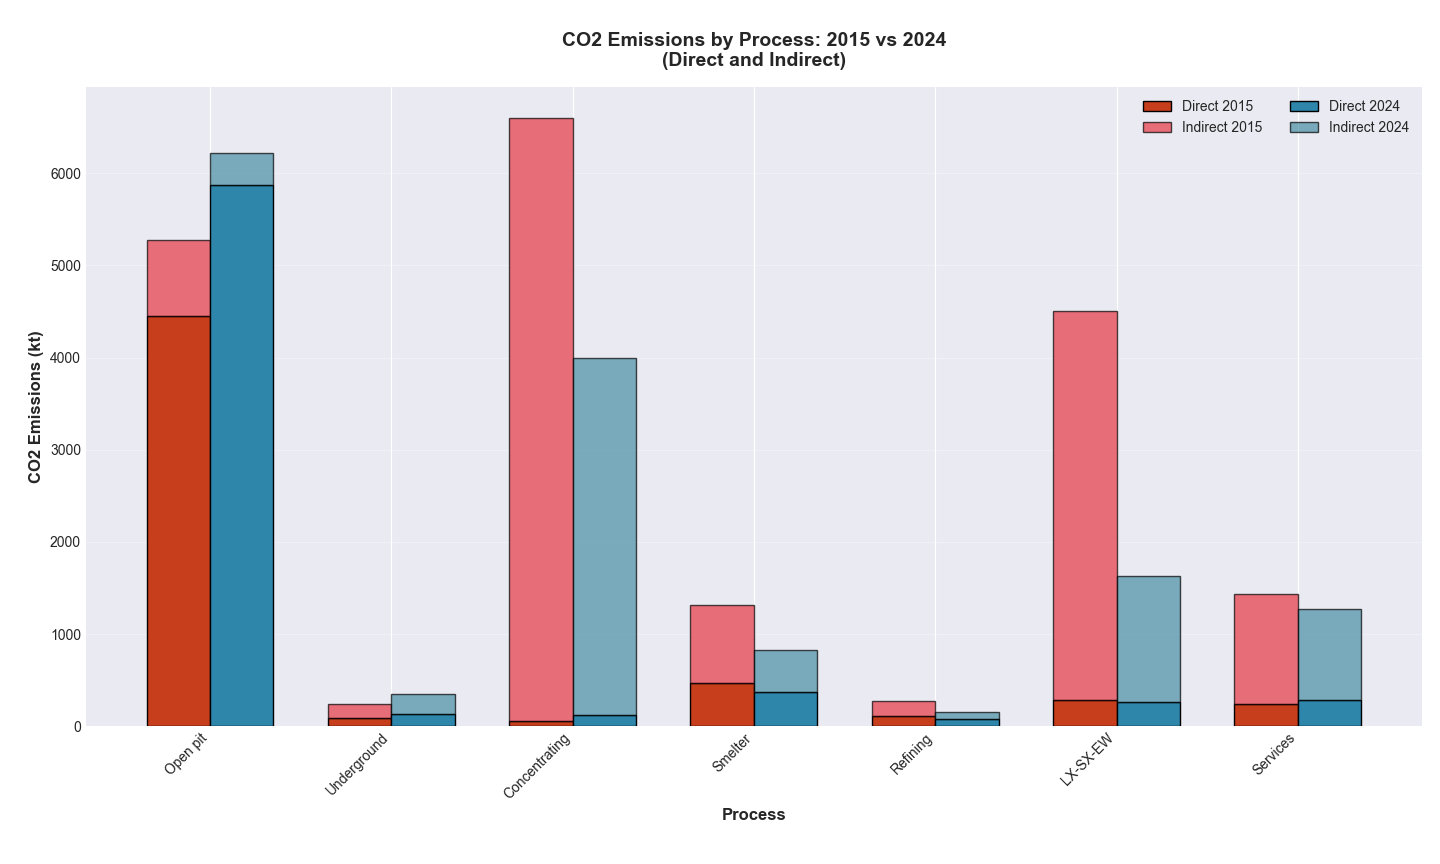
\includegraphics[width=0.9\linewidth]{Figures/Figure_6.png}
    \caption{CO$_2$ emissions by process (2015 vs 2024)}
\end{figure}
This figure compares greenhouse gas emissions for each process and decomposes them into direct emissions (fuel combustion) and indirect emissions (electricity consumption). It is clear that the most polluting processes are open-pit mining, concentrating, and the LX-SX-EW process. Apart from open-pit mining, the share of emissions originating from fuel combustion has remained relatively constant over the years, while emissions associated with electricity consumption have decreased significantly, particularly for concentrating and LX-SX-EW. The graph clearly shows that open-pit mining has a major impact on total emissions. Unlike the other processes, its emissions have increased rather than decreased over time. This is mainly because it is the only process in which fuel consumption represents a very large share of total energy use. These results suggest that electrifying open-pit mining activities, or reducing reliance on fuel intensive machinery, could represent one of the most effective levers for decarbonizing the copper production sector. From a broader perspective, each process has a distinct impact on total emissions, and the balance between direct and indirect emissions varies significantly across processes. As discussed in Section \ref{sec:heterogeneity}, emissions are highly heterogeneous throughout the production chain, making it essential to analyze each process separately.
\subsection{Opportunities for Decarbonization}
\label{sec:opportunities}
From the different figures that we have analyzed above, we have seen that CO$_2$ has decreased mainly due to grid decarbonization, which clearly relies on the fact that renewable sources represented nearly 70\% of Chile's electricity generation (Section \ref{sec:elec & renew}). It is thus very important that Chile continues to transition toward renewable resources.
\
As mentioned in Section \ref{sec:emissions by process}, the main lever to reduce CO$_2$ emissions is working on how to replace current machinery. Loading and hauling are among the major sources of greenhouse gas emissions in open-pit mining, so shifting from fuel-based transportation methods to electricity-based ones can be very impactful.
\
Therefore, replacing fuel haul-trucks with battery-electric or electric road system trucks can reduce CO$_2$ emissions significantly. Electric road systems are similar to trolley buses, meaning that trucks are powered by overhead lines. A simulation study by \textit{Lindgren et al., 2022} examined the feasibility of large battery-electric haul trucks using Aitik copper mine in Sweden. They concluded that compared to classic operation, electric haul trucks could increase productivity by 16\% while reducing costs by 44\%. \cite{Simulations_of_Battery_Electric} This suggests that apart from an environmental perspective, shifting toward electrified trucks also has economic value, which is very important because it increases the likelihood that large mining companies will invest in these technologies.
\
We also wanted to look concretely at what types of solutions are available on the market to decarbonize the sector. Liebherr, a Swiss equipment manufacturer, operates diesel-electric haul trucks equipped with the Trolley Assist System (Liebherr T 284) in the open pit of Collahuasi and has installed a 1 km trolley line. This results in a 26\% decrease in fuel consumption and a 94\% decrease in CO$_2$ emissions on the ramp. The company also offers electric mining excavators. They are also developing trucks with battery-electric powertrains and trucks operating with alternative fuels such as ammonia and hydrogen.\cite{Liebherr} However, loading and hauling represent more than 50\% of total mine input costs. This suggests that moving toward new machinery is very expensive and a complete fleet cannot be replaced easily.\cite{Mining_fleet_management}
    \newpage
\section{Carbon Intensity of Electricity and the Chilean Energy Transition}
    The Kaya decomposition presented in Section \ref{sec:decomposition} identifies $\text{CI}_{\text{elec}}$, the carbon intensity of electricity, as one of the most actionable levers for reducing CO$_2$ emissions from copper production. Unlike ore grade, which is a geological constraint, $\text{CI}_{\text{elec}}$ responds directly to energy policy and investment decisions. This has an important implication for electrification: replacing diesel and fossil fuels with electricity across the copper production chain only reduces emissions if the electricity itself is low-carbon. On a coal-heavy grid, electrification can actually worsen the carbon footprint, as indirect emissions from power generation may exceed the savings from cutting on-site combustion. This section examines why Chile is increasingly moving away from this risk, and why the conditions for productive electrification are now largely in place.

\subsection{Historical Evolution of the Electricity Mix}

\subsubsection{Geographic Foundations of the Energy Transition}

Chile's renewable energy potential is largely a product of its geography. The country stretches over 4,300~km from north to south, which places very different climatic zones within the same national grid.

\begin{figure}[H]
    \centering
    \begin{minipage}{0.48\textwidth}
        \centering
        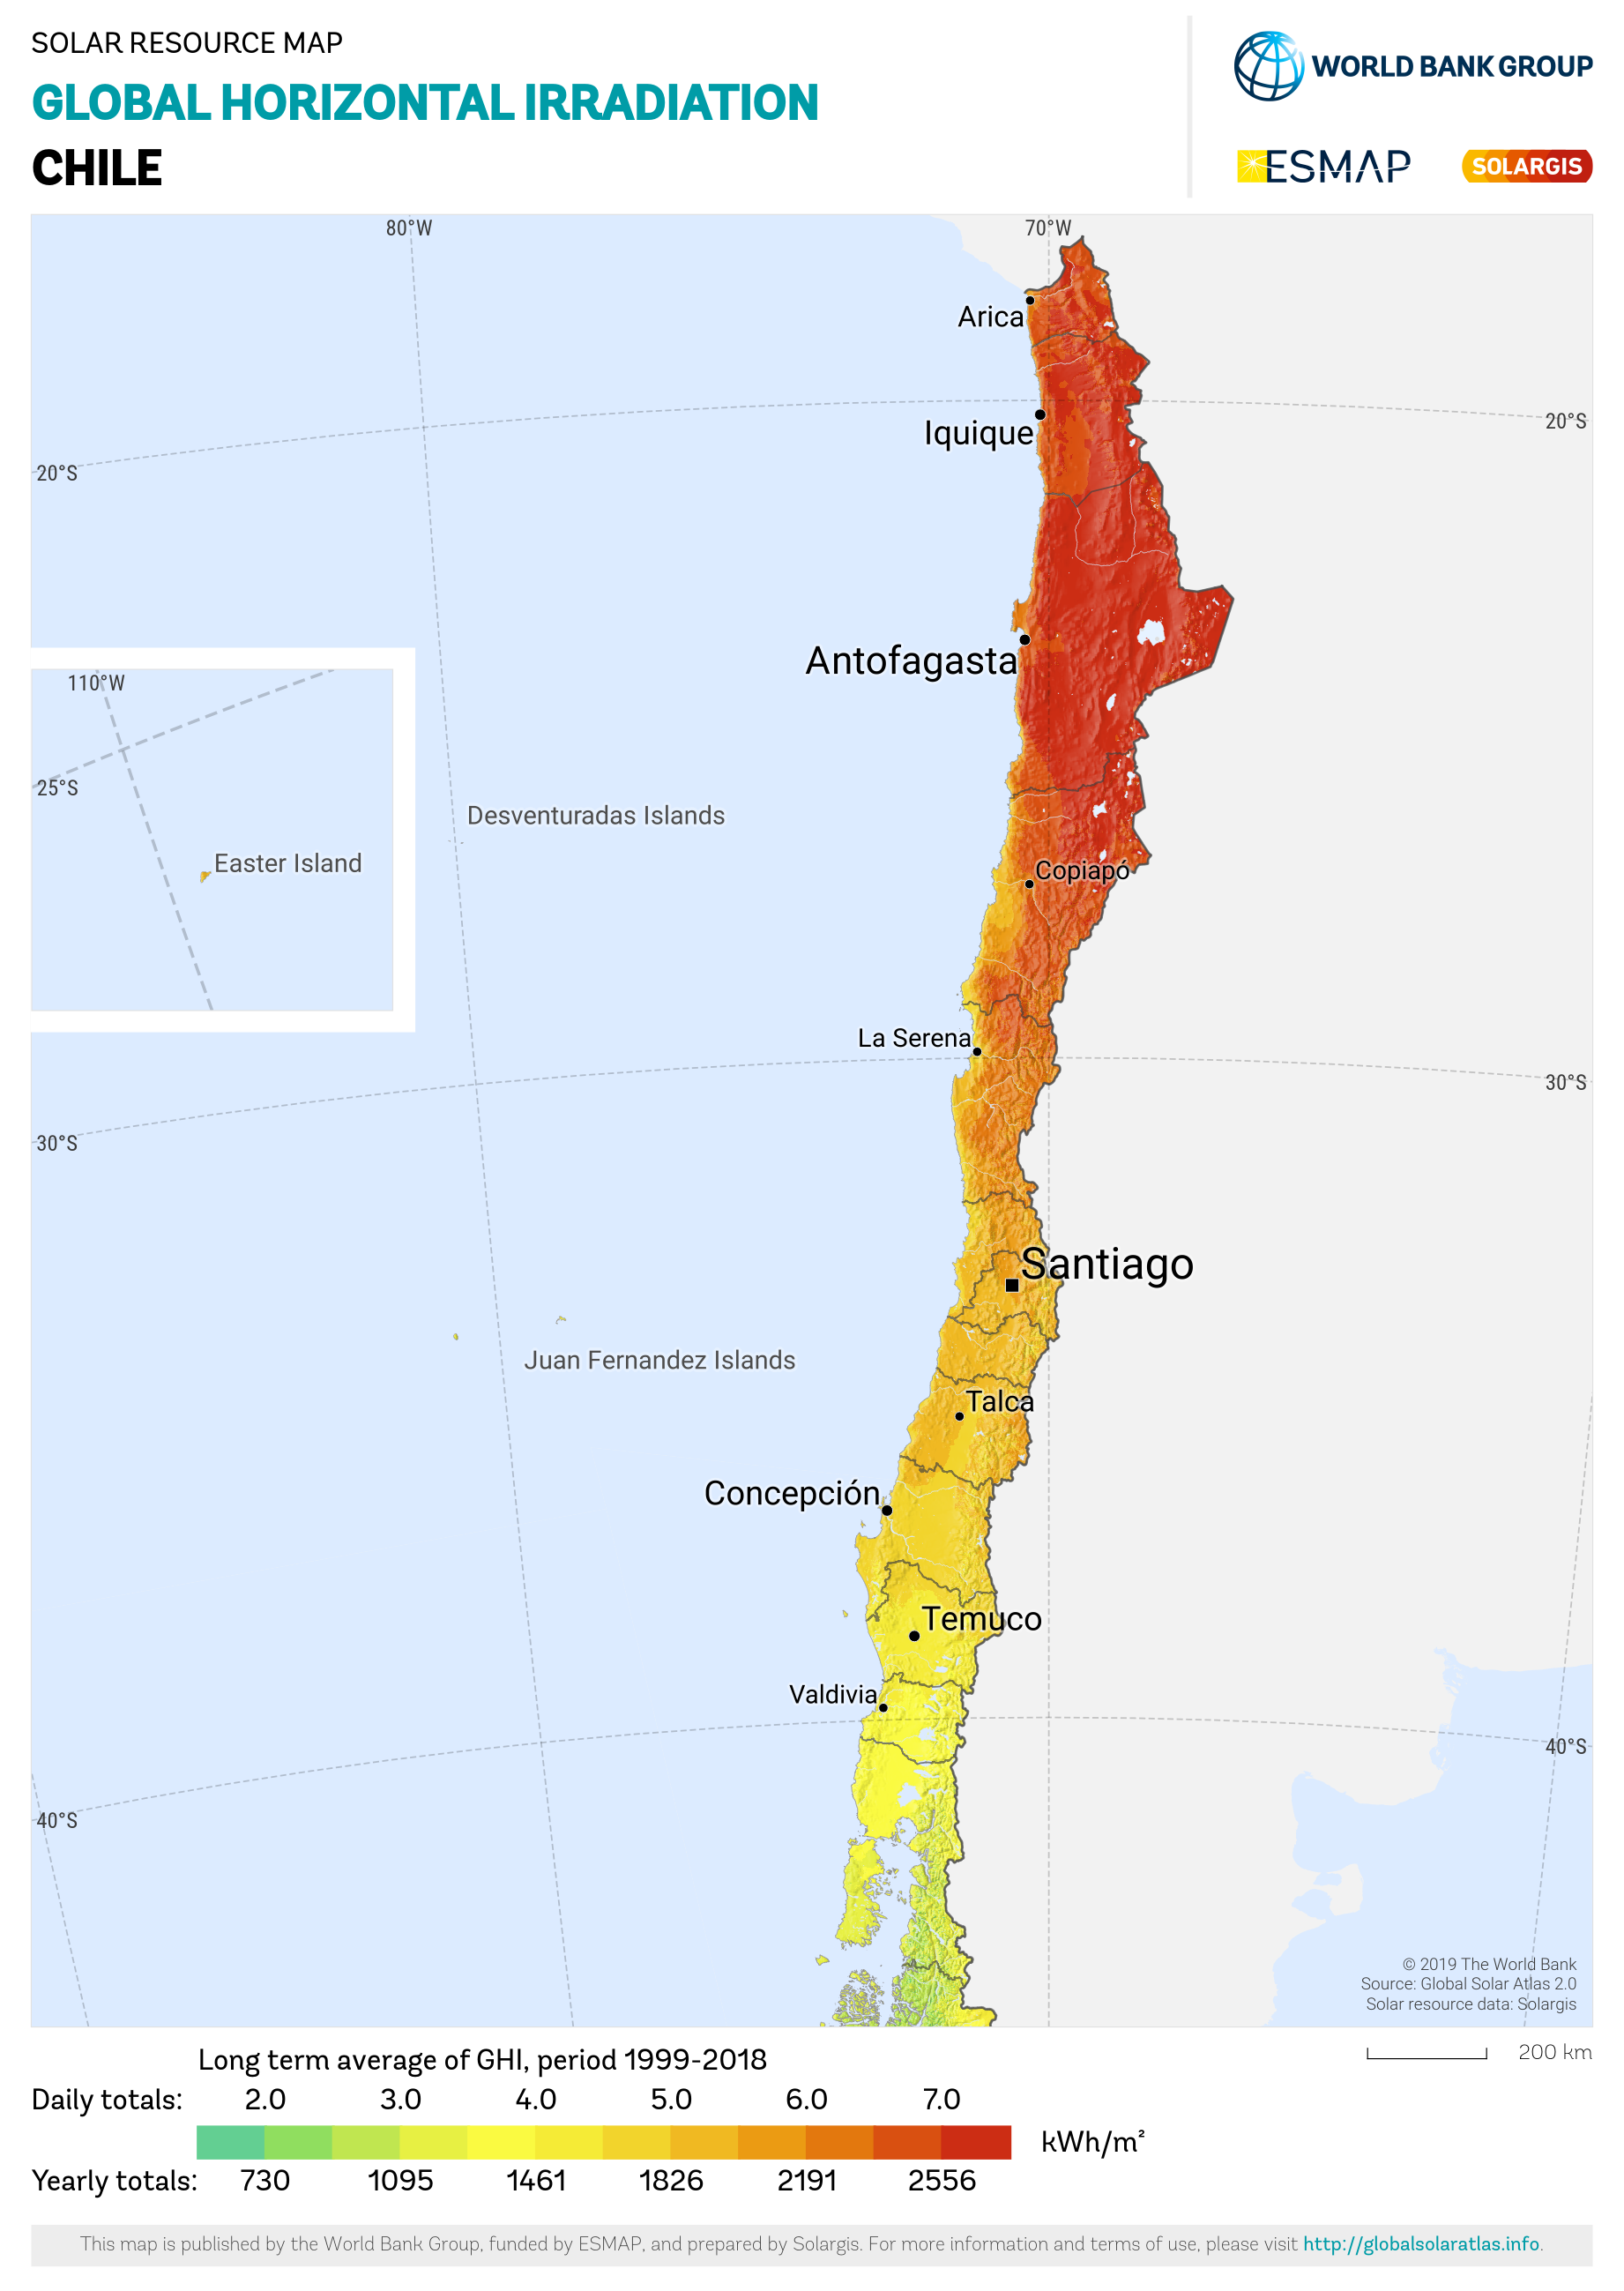
\includegraphics[width=\linewidth]{Figures/Chile_GHI_mid-size-map_156x220mm-300dpi_v20191015.png}
        \caption{Global Horizontal Irradiation (GHI) in Chile, long-term average 1999--2018 (kWh/m$^2$). \textcopyright~2019 The World Bank, Source: Global Solar Atlas~2.0, Solar resource data: Solargis.}
        \label{fig:ghi_map}
    \end{minipage}
    \hfill
    \begin{minipage}{0.48\textwidth}
        \centering
        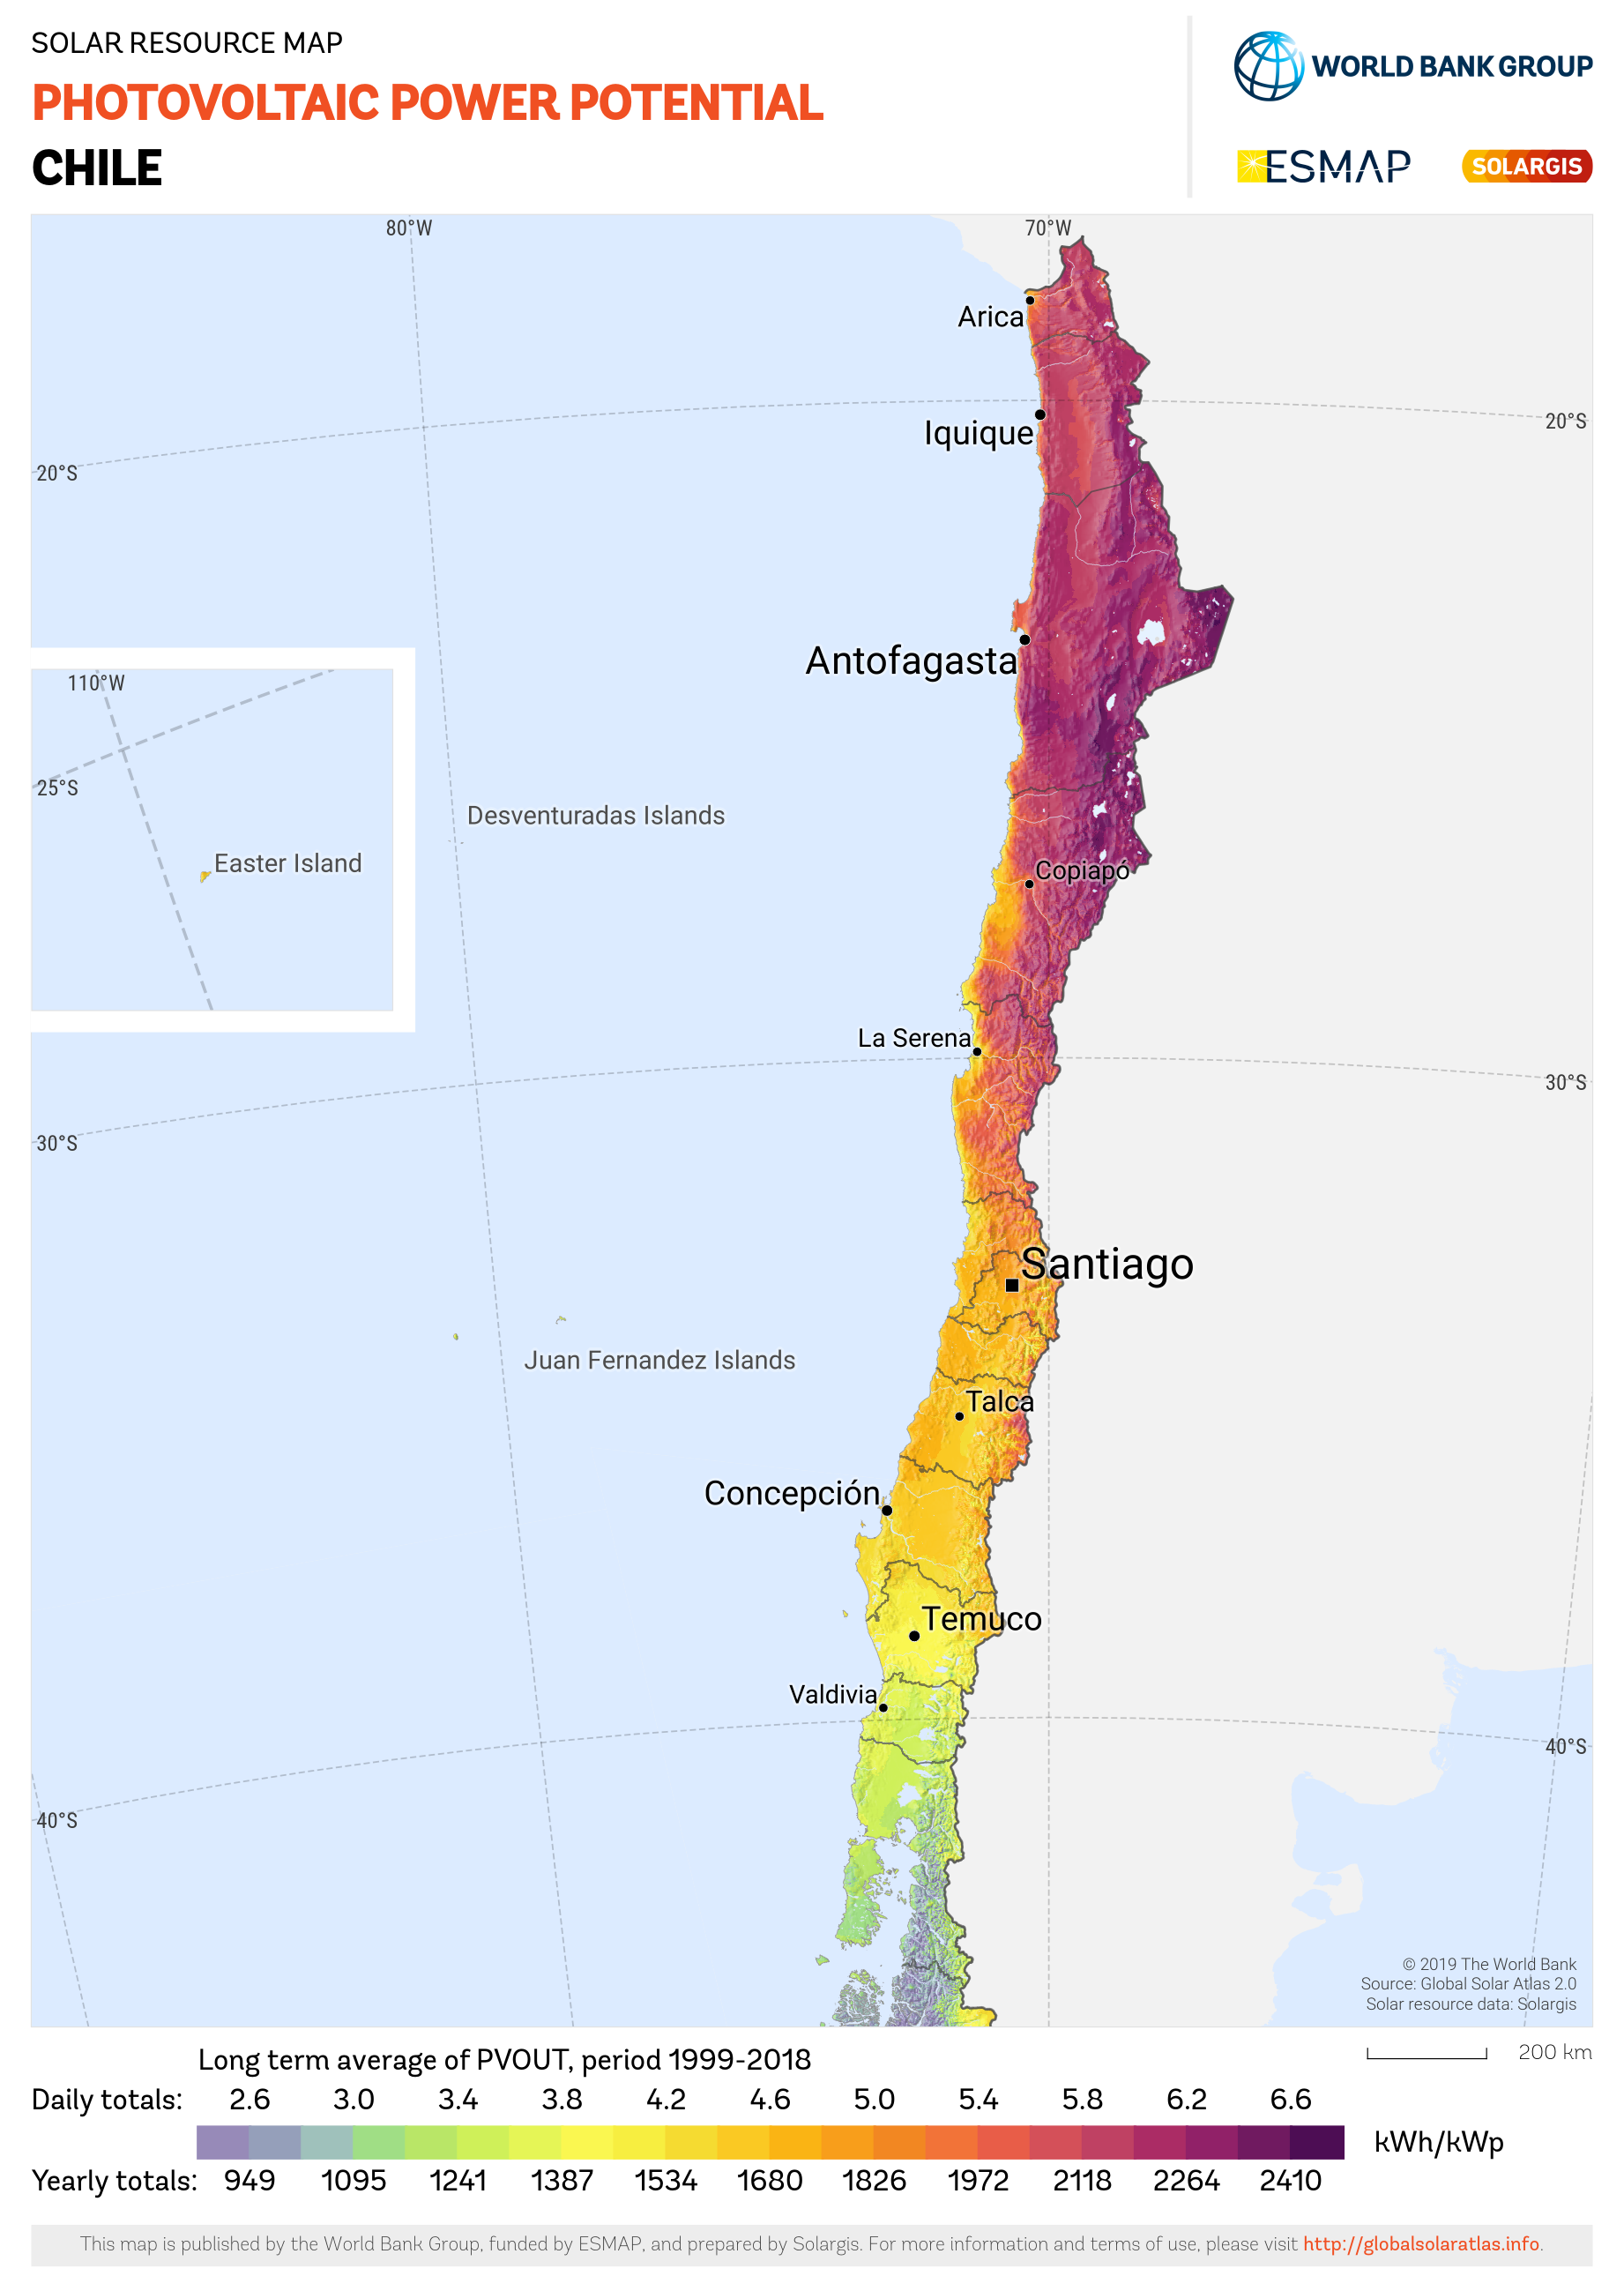
\includegraphics[width=\linewidth]{Figures/Chile_PVOUT_mid-size-map_156x220mm-300dpi_v20191015.png}
        \caption{Photovoltaic power potential (PVOUT) in Chile, long-term average 1999--2018 (kWh/kWp). \textcopyright~2019 The World Bank, Source: Global Solar Atlas~2.0, Solar resource data: Solargis.}
        \label{fig:pvout_map}
    \end{minipage}
\end{figure}

\begin{figure}[H]
    \centering
    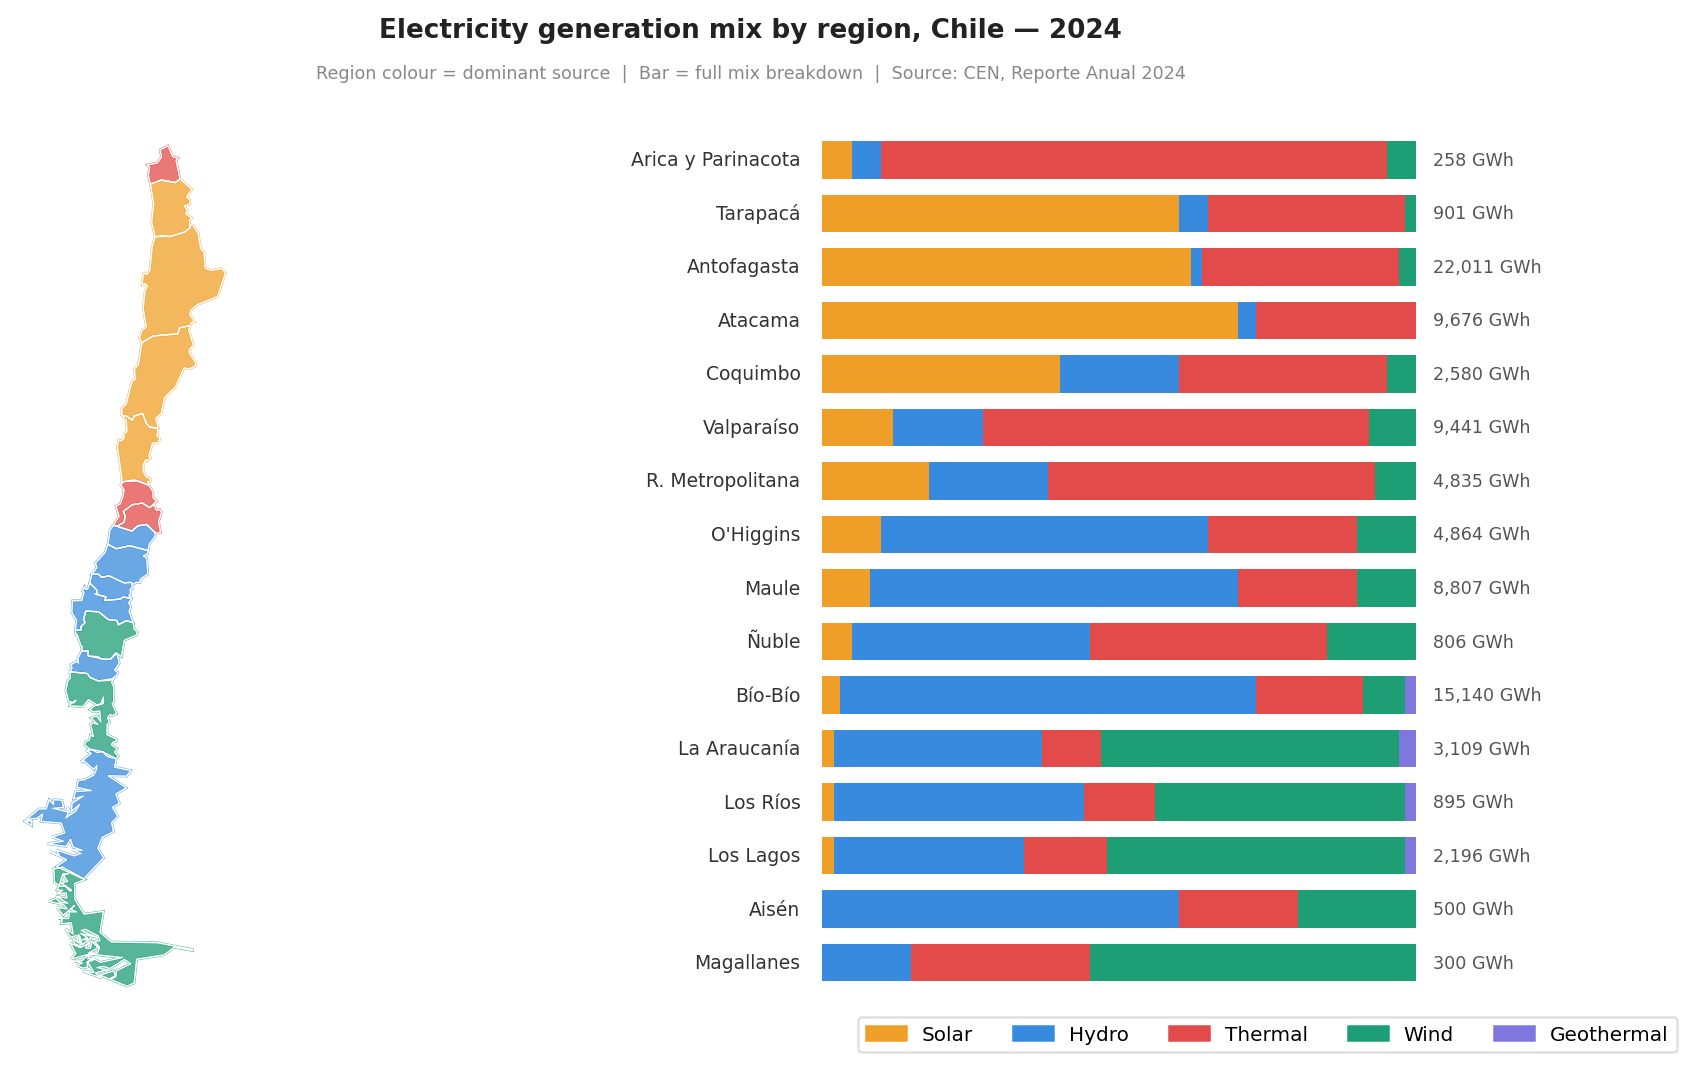
\includegraphics[width=0.72\linewidth]{Figures/chile_energy_map.png}
    \caption{Electricity generation mix by region in Chile, 2024. Each region is coloured by its dominant source; horizontal bars show the full breakdown, with output in GWh. Source: Coordinador Eléctrico Nacional, Reporte Anual 2024.}
    \label{fig:cen_region}
\end{figure}

As Figure~\ref{fig:cen_region} illustrates, Chile's geography creates three broadly distinct renewable energy zones \cite{SolarAtlas2019}. The northern desert, with Global Horizontal Irradiance values regularly exceeding 2,500~kWh/m$^2$/year, is dominated by solar photovoltaic. The central zone relies primarily on hydropower, drawing on the river systems fed by Andean snowmelt. The south benefits from strong and consistent winds, making it one of the most promising onshore wind corridors in the world. These three resources peak at different times of day and year, which makes them a good fit for each other within a single grid.

\subsubsection{From Coal Dominance to Renewable Leadership (2000--2024)}

Between 2000 and 2013, Chile expanded its coal-fired capacity to keep pace with rapid demand growth, and the carbon intensity of the grid rose accordingly, reaching approximately 482~gCO$_2$/kWh in 2013 \cite{IEAChile2024}. Coal still accounted for 43.6\% of electricity output as late as 2016 \cite{ProgressPlaybook2024}. The shift began around 2014--2015, when falling costs for solar PV and wind, combined with resistance from local communities to new thermal projects, started to alter the investment landscape. The pace of change accelerated after 2019, as shown in Figure~\ref{fig:owid_mix}.

\begin{figure}[H]
    \centering
    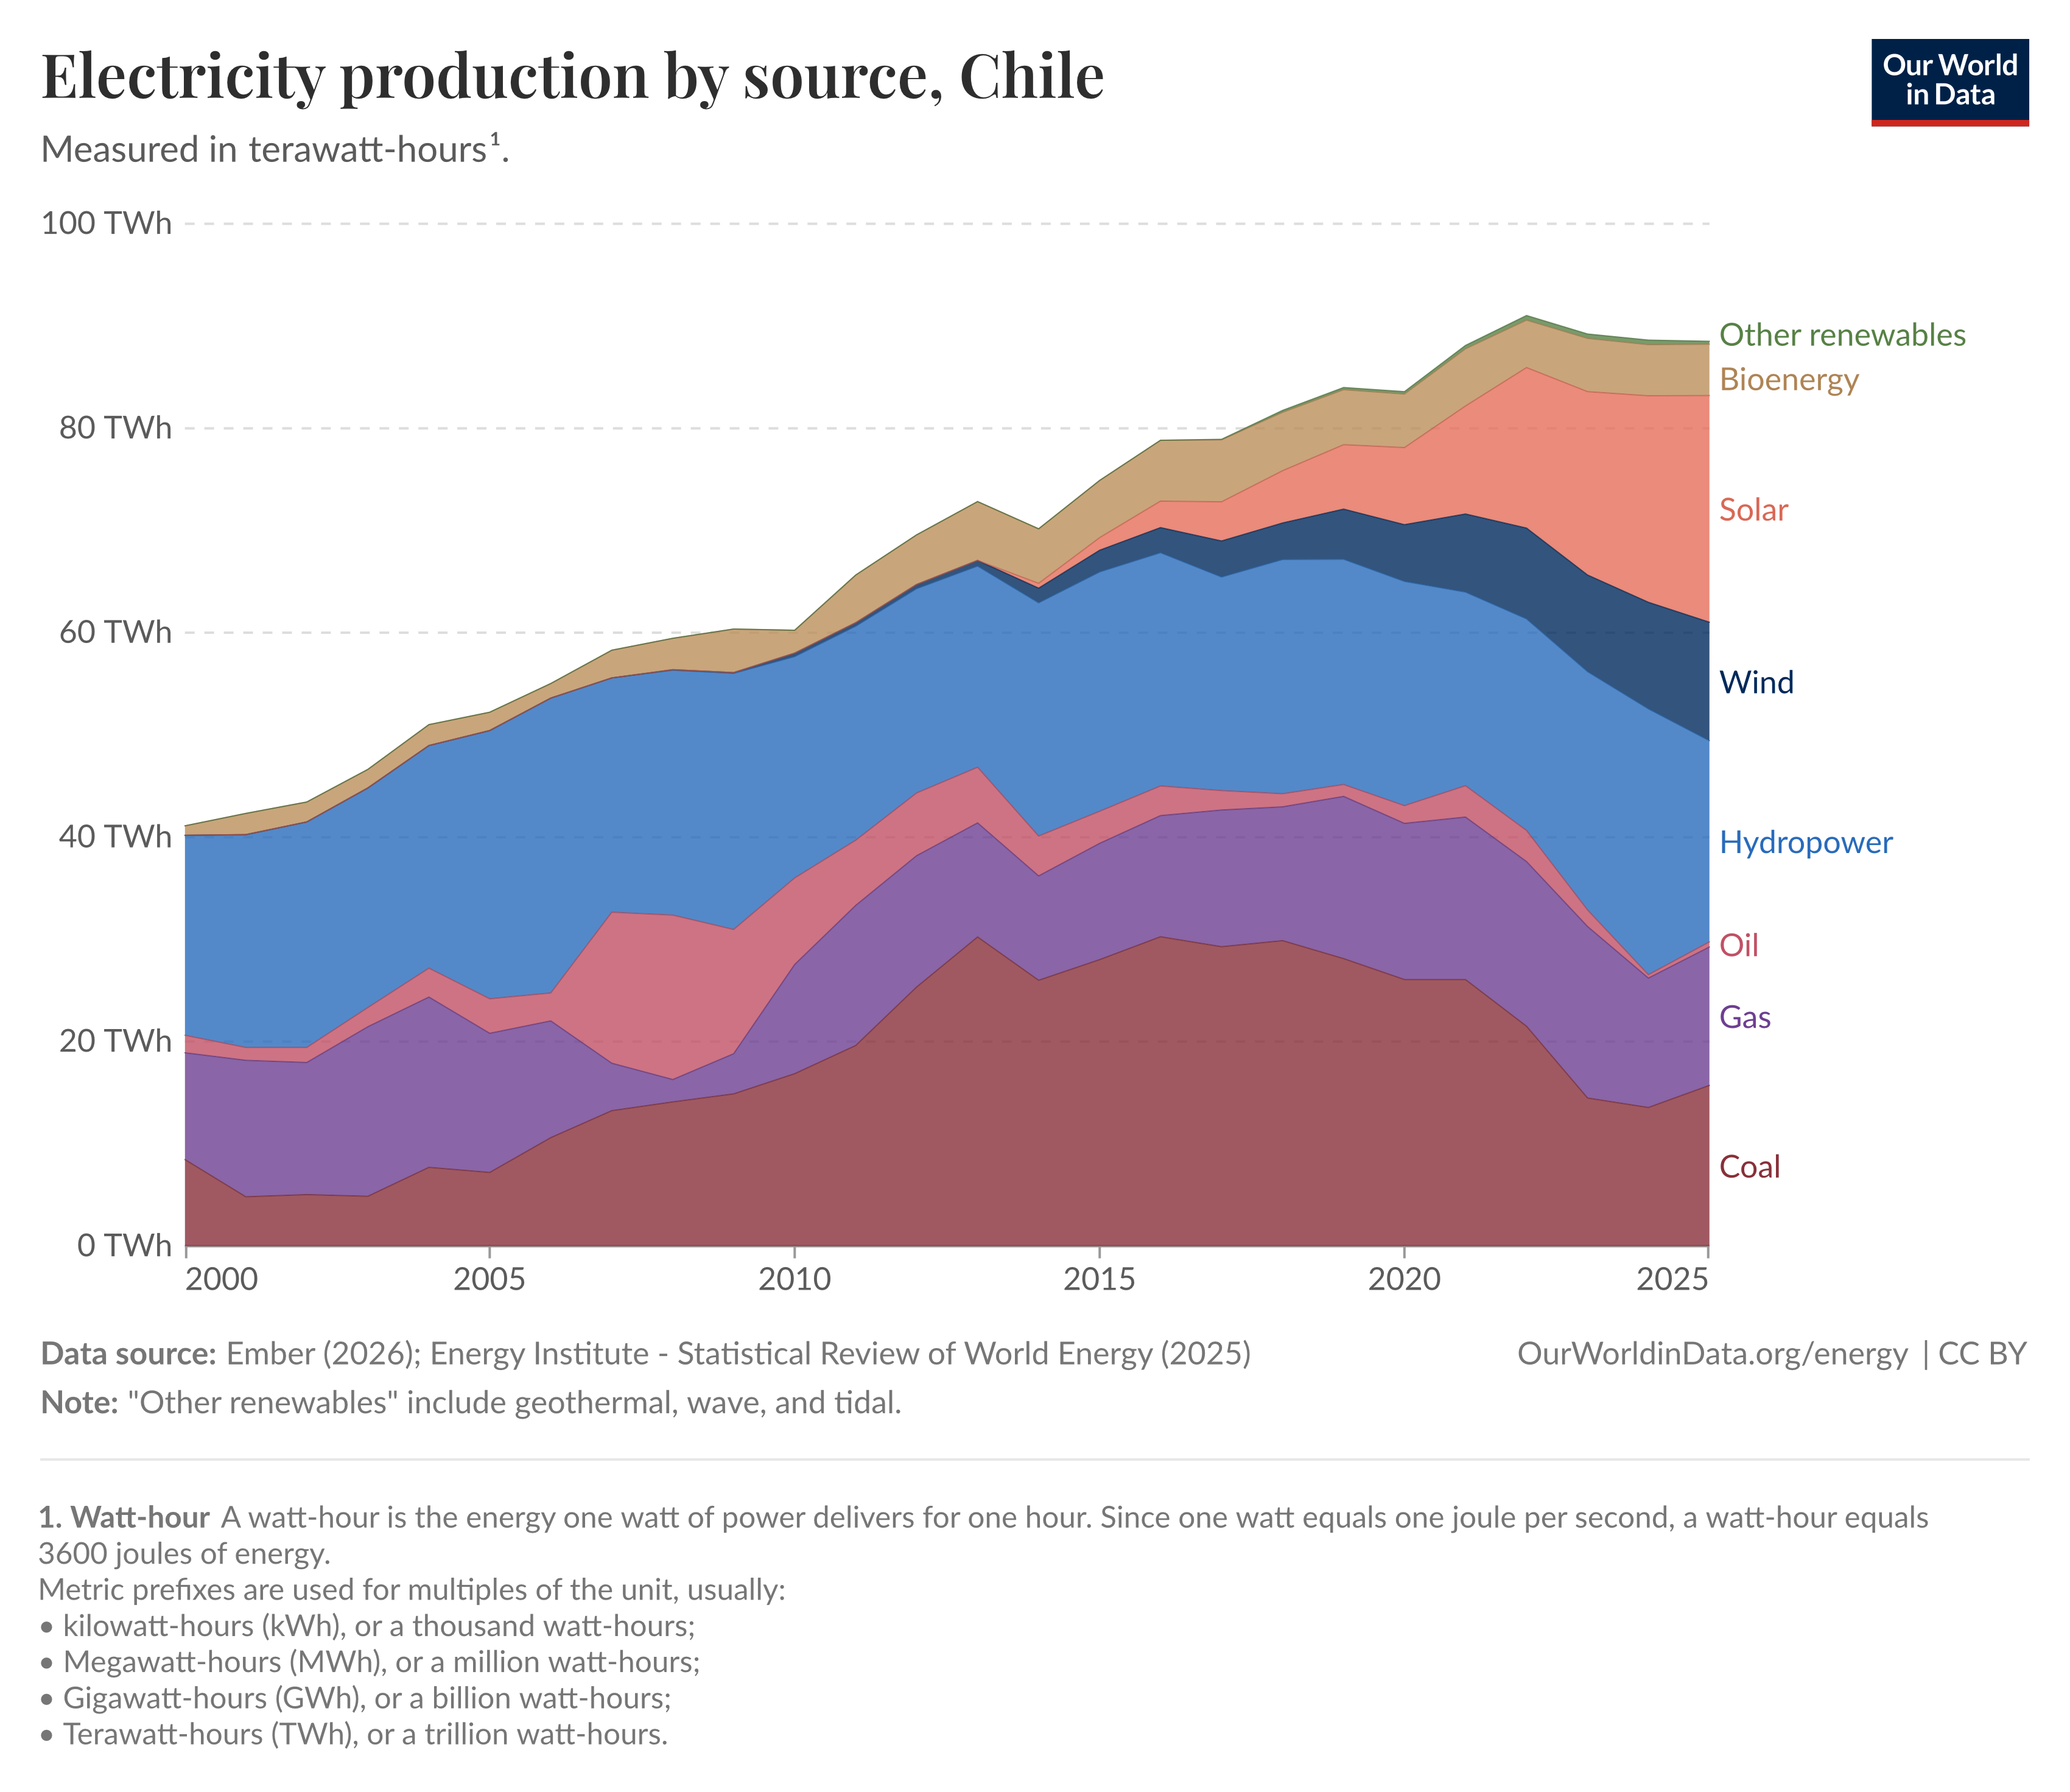
\includegraphics[width=0.85\linewidth]{Figures/electricity-prod-source-stacked.png}
    \caption{Electricity production by source in Chile, 2000--2025 (TWh). Source: Our World in Data, based on Ember (2026) and Energy Institute -- Statistical Review of World Energy (2025) \cite{OWID2026}.}
    \label{fig:owid_mix}
\end{figure}

By 2024, renewables accounted for roughly 70\% of national electricity generation, while coal had retreated to 14\% \cite{EnergiaEstrategica2025}. Solar and wind together provided 35\% of generation that year, compared to 14\% in 2019 \cite{Ember2025}. Solar energy alone reached 19.92~TWh, or 22.3\% of total national output, up from less than 0.1\% in 2013 \cite{WikipediaSolar2025}.

These shifts in the generation mix translated directly into a lower $\text{CI}_{\text{elec}}$. From IEA data on power sector emissions and total production, we compute that the carbon intensity of Chilean electricity fell from its 2013 peak of 482~gCO$_2$/kWh to 221~gCO$_2$/kWh in 2023, a reduction of over 54\% in ten years. The industry body Generadoras de Chile reports a consistent picture using the national grid emissions factor, which declined from 0.53~tCO$_2$/MWh in 2013 to 0.20~tCO$_2$/MWh in 2024, a 63\% drop over the same period. At the national level, energy-related CO$_2$ emissions peaked at 94~Mt in 2019 and had fallen by over 20\% to 72~Mt by 2024 \cite{IEAChile2026}.

\begin{figure}[H]
    \centering
    \begin{minipage}{0.48\textwidth}
        \centering
        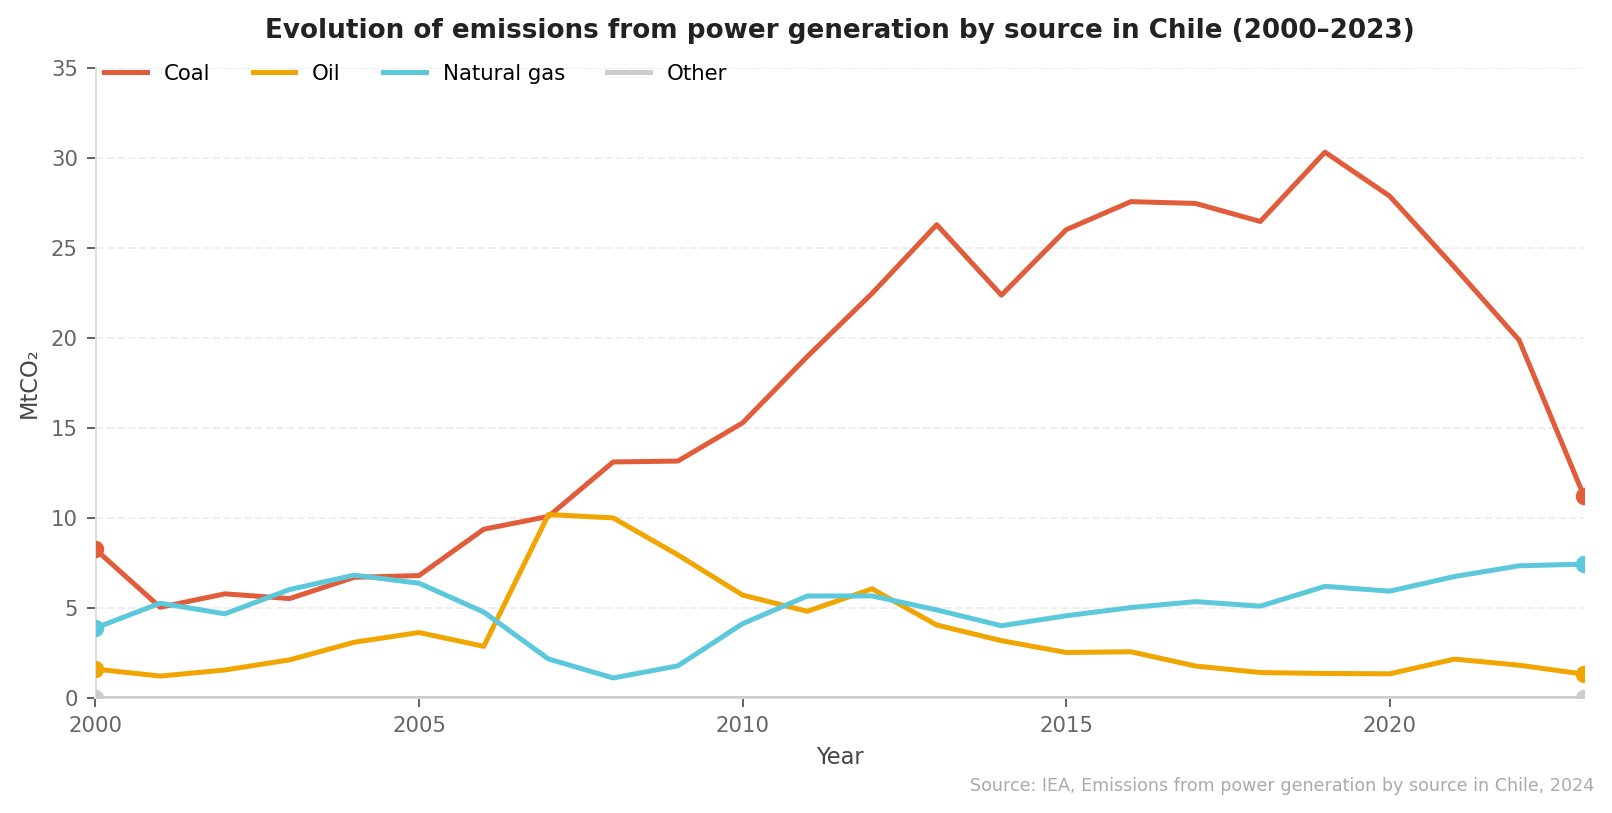
\includegraphics[width=\linewidth]{Figures/chile_emissions_by_source.png}
        \caption{CO$_2$ emissions from power generation by source in Chile, 2000--2023 (MtCO$_2$). Source: IEA, authors' calculations.}
        \label{fig:emissions_source}
    \end{minipage}
    \hfill
    \begin{minipage}{0.48\textwidth}
        \centering
        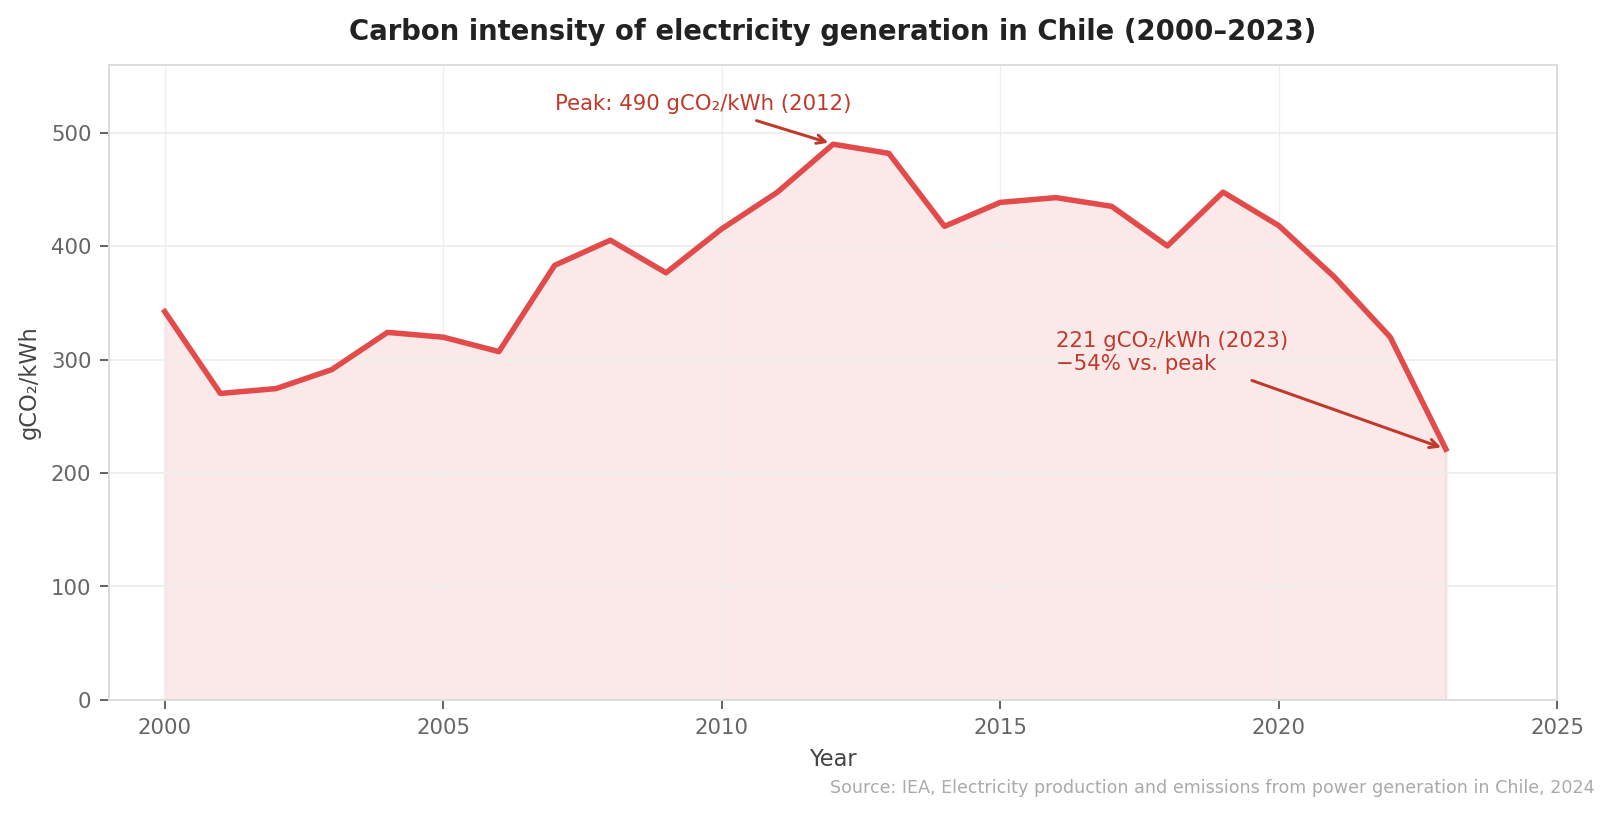
\includegraphics[width=\linewidth]{Figures/chile_ci_elec.png}
        \caption{Carbon intensity of electricity generation in Chile, 2000--2023 (gCO$_2$/kWh). Source: IEA, authors' calculations.}
        \label{fig:ci_elec}
    \end{minipage}
\end{figure}

Figures~\ref{fig:emissions_source} and~\ref{fig:ci_elec} show the same trend from two angles. The fall in coal-fired generation cut the grid's carbon intensity roughly in half, from a peak of 482~gCO$_2$/kWh in 2013 to 221~gCO$_2$/kWh in 2023. On the capacity side, eleven coal plants have been retired since 2018, removing 1,679~MW from the grid, while over 19,000~MW of renewable generation and storage capacity have been added over the same period. As of November 2024, ERNC capacity totalled 16,422~MW in the SEN, representing 47.4\% of total installed capacity across all national electricity systems \cite{CNE2024}. Solar PV accounts for 29.9\% of this total and wind for 13.6\%, with both technologies still expanding rapidly.

\subsection{Political Commitments and Legal Framework}

Chile's energy transition is backed by a fairly solid legal and political framework. In 2020, Chile submitted an updated Nationally Determined Contribution (NDC) to the UNFCCC, committing to cap greenhouse gas emissions at 95~MtCO$_2$e by 2030 and to peak emissions no later than 2025, with a binding objective of carbon neutrality by 2050 \cite{CAT2020}. The Climate Action Tracker rates Chile's overall targets as ``Almost Sufficient'', meaning the ambition is above average by international standards but still falls short of full alignment with the 1.5°C pathway.

On the electricity side, the government has been more concrete. Since 2018, eleven coal plants have been voluntarily shut down under agreements between the government and the main utilities, ahead of any legal requirement to do so. A broader coal phase-out by 2040 is now government policy, with proposals circulating to bring that deadline forward to 2035, and the Energy Transition Act passed in December 2024 strengthens the legal basis for accelerating renewable deployment and integrating storage into the grid \cite{GLI2026}.

For copper mining, these commitments are particularly relevant: the sector consumes close to 30\% of Chile's national electricity \cite{Cochilco2024}, so any drop in the grid's carbon intensity reduces mining emissions automatically, even before any changes are made at the mine level.

\subsection{Projections and Implications for Copper Electrification}

According to the IEA's 2050 Energy Transition Roadmap for Chile, the carbon intensity of the grid is expected to fall from around 189~gCO$_2$/kWh today to 29~gCO$_2$/kWh by 2035, as coal is phased out and renewables continue to expand. As shown in Figure~\ref{fig:ci_elec_proj}, this would represent a reduction of over 85\% compared to the 2013 peak.

\begin{figure}[H]
    \centering
    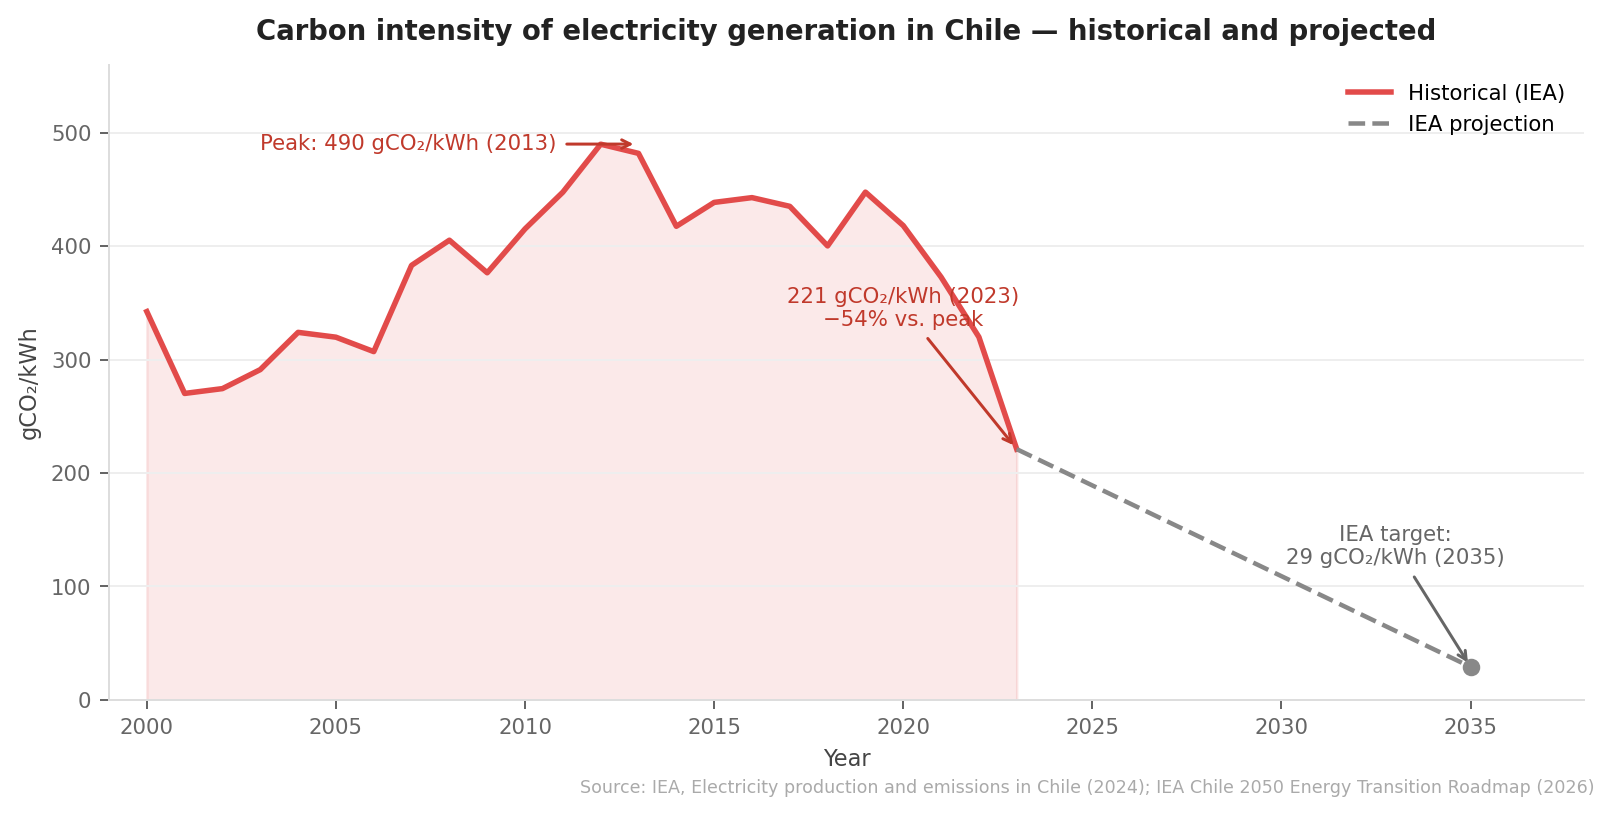
\includegraphics[width=0.85\linewidth]{Figures/chile_ci_elec_projection.png}
    \caption{Carbon intensity of electricity generation in Chile, historical and projected (gCO$_2$/kWh). Source: IEA.}
    \label{fig:ci_elec_proj}
\end{figure}

At 29~gCO$_2$/kWh, the indirect emissions from grid electricity become small compared to the direct emissions from burning diesel or gas on-site. Electrifying operations such as haulage, crushing, or concentration would then produce real emission reductions rather than simply shifting them from one source to another. The grid is already clean enough to make this worthwhile, and the trend is set to continue.
    \newpage
\section{Conclusion}
Between 2015 and 2024, CO$_2$ emissions from Chilean copper production fell by roughly 17\% despite a sustained increase in energy consumption. The decomposition analysis shows that this was not the result of technological improvements in mining itself. The carbon intensity of combustion fuels stayed roughly constant over the period, and the share of electricity in total energy use barely moved. What changed was the electricity grid: as coal was progressively replaced by solar and wind, the carbon intensity of electricity fell by over 37\%, pulling down indirect emissions with it.

This matters for how we interpret the current situation. The progress made so far has come largely for free from a mining perspective, driven by Chile's broader energy transition rather than by anything the sector has done differently. Direct emissions, which come mainly from diesel-powered machinery in open-pit operations, actually increased over the period. As ore grades continue to decline and extraction goes deeper, this pressure will only grow.

The path forward depends on two things happening together. First, the grid needs to keep decarbonizing. The IEA projects a carbon intensity of 29~gCO$_2$/kWh by 2035, down from around 189 today. At that level, electrifying haul trucks or concentrating plants would produce emission reductions, not just a change in where the emissions are counted. Second, the sector itself needs to start shifting away from diesel. That transition is expensive and slow replacing a mining fleet takes years and significant capital but section \ref{sec:opportunities} shows there are already viable technologies on the market. The two conditions reinforce each other: a cleaner grid makes the investment in electrification more worthwhile, and electrification makes the grid decarbonization more impactful for copper emissions.

Chile's geography is an asset in this respect. The northern desert, where most of the country's copper is mined, also has some of the highest solar irradiance in the world. The conditions for a low-carbon copper industry are better here than almost anywhere else. The question is whether the investment follows.
\section{Use of AI}
The use of artificial intelligence in this report was to improve the clarity, grammar, spelling, and overall readability of the English text. The tool supported us by identifying linguistic errors, suggesting more natural phrasing, and helping ensure consistency in terminology and sentence structure throughout the document. The use of AI was limited to language refinement only and did not contribute to the scientific content, data analysis, interpretation of results, or conclusions presented in this study. All final revisions and approval of the manuscript content were performed by us.
\newpage
\bibliographystyle{abbrv}
\bibliography{References.bib}
\end{document}
